%% FHNW Thesis template
% Template version used: v1.0
%
% Largely adapted from Adrian Nievergelt's template for the ADPS
% (lecture notes) project. Downloaded and further adapted from
% https://www.cadmo.ethz.ch/education/thesis/template.html


%% We use the memoir class because it offers a many easy to use features.
\documentclass[11pt,a4paper,titlepage]{memoir}

%% Packages
%% ========

%% LaTeX Font encoding -- DO NOT CHANGE
\usepackage[OT1]{fontenc}

%% Babel provides support for languages.  'english' uses British
%% English hyphenation and text snippets like "Figure" and
%% "Theorem". Use the option 'ngerman' if your document is in German.
%% Use 'american' for American English.  Note that if you change this,
%% the next LaTeX run may show spurious errors.  Simply run it again.
%% If they persist, remove the .aux file and try again.
\usepackage[german]{babel}

%% Input encoding 'utf8'. In some cases you might need 'utf8x' for
%% extra symbols. Not all editors, especially on Windows, are UTF-8
%% capable, so you may want to use 'latin1' instead.
\usepackage[utf8]{inputenc}

%% This changes default fonts for both text and math mode to use Herman Zapfs
%% excellent Palatino font.  Do not change this.
\usepackage[sc]{mathpazo}

%% The AMS-LaTeX extensions for mathematical typesetting.  Do not
%% remove.
\usepackage{amsmath,amssymb,amsfonts,mathrsfs}

%% NTheorem is a reimplementation of the AMS Theorem package. This
%% will allow us to typeset theorems like examples, proofs and
%% similar.  Do not remove.
%% NOTE: Must be loaded AFTER amsmath, or the \qed placement will
%% break
\usepackage[amsmath,thmmarks]{ntheorem}

%% We unfortunately need this for the Rules chapter.  Remove it
%% afterwards; or at least NEVER use its underlining features.
\usepackage{soul}

%% This allows you to add .pdf files. It is used to add the
%% declaration of originality.
\usepackage{pdfpages}

%% Some more packages that you may want to use.  Have a look at the
%% file, and consult the package docs for each.
%% See the TeXed file for more explanations

%% [OPT] Multi-rowed cells in tabulars
%\usepackage{multirow}

%% [REC] Intelligent cross reference package. This allows for nice
%% combined references that include the reference and a hint to where
%% to look for it.
\usepackage{varioref}

%% [OPT] Easily changeable quotes with \enquote{Text}
%\usepackage[german=swiss]{csquotes}

%% [REC] Format dates and time depending on locale
\usepackage{datetime}

%% [OPT] Provides a \cancel{} command to stroke through mathematics.
%\usepackage{cancel}

%% [NEED] This allows for additional typesetting tools in mathmode.
%% See its excellent documentation.
\usepackage{mathtools}

% Acronym
\usepackage[nohyperlinks, printonlyused, withpage, smaller]{acronym}

%% [ADV] Conditional commands
%\usepackage{ifthen}

%% [OPT] Manual large braces or other delimiters.
%\usepackage{bigdelim, bigstrut}

%% [REC] Alternate vector arrows. Use the command \vv{} to get scaled
%% vector arrows.
\usepackage[h]{esvect}

%% [NEED] Some extensions to tabulars and array environments.
\usepackage{array}

%% [OPT] Postscript support via pstricks graphics package. Very
%% diverse applications.
%\usepackage{pstricks,pst-all}

%% [?] This seems to allow us to define some additional counters.
%\usepackage{etex}

%% [ADV] XY-Pic to typeset some matrix-style graphics
%\usepackage[all]{xy}

%% [OPT] This is needed to generate an index at the end of the
%% document.
%\usepackage{makeidx}

%% [OPT] Fancy package for source code listings.  The template text
%% needs it for some LaTeX snippets; remove/adapt the \lstset when you
%% remove the template content.
\usepackage{listings}
\usepackage{color}

\definecolor{dkgreen}{rgb}{0,0.6,0}
\definecolor{gray}{rgb}{0.5,0.5,0.5}
\definecolor{mauve}{rgb}{0.58,0,0.82}

\lstset{frame=tb,
language=Java,
aboveskip=3mm,
belowskip=3mm,
showstringspaces=false,
columns=flexible,
basicstyle={\small\ttfamily},
numbers=none,
numberstyle=\tiny\color{gray},
keywordstyle=\color{blue},
commentstyle=\color{dkgreen},
stringstyle=\color{mauve},
breaklines=true,
breakatwhitespace=true,
tabsize=3
}

%% [REC] Fancy character protrusion.  Must be loaded after all fonts.
\usepackage[activate]{pdfcprot}

%% [REC] Nicer tables.  Read the excellent documentation.
\usepackage{threeparttable}
\usepackage{booktabs}

% [REC] Quotes
\usepackage{natbib}


%% Our layout configuration.  DO NOT CHANGE.
%% Memoir layout setup

%% NOTE: You are strongly advised not to change any of them unless you
%% know what you are doing.  These settings strongly interact in the
%% final look of the document.

% Dependencies
\usepackage{FHNWlogo}

% Turn extra space before chapter headings off.
\setlength{\beforechapskip}{0pt}

\nonzeroparskip
\parindent=0pt
\defaultlists

% Chapter style redefinition
\makeatletter

\if@twoside
  \pagestyle{Ruled}
  \copypagestyle{chapter}{Ruled}
\else
  \pagestyle{ruled}
  \copypagestyle{chapter}{ruled}
\fi
\makeoddhead{chapter}{}{}{}
\makeevenhead{chapter}{}{}{}
\makeheadrule{chapter}{\textwidth}{0pt}
\copypagestyle{abstract}{empty}

\makechapterstyle{bianchimod}{%
  \chapterstyle{default}
  \renewcommand*{\chapnamefont}{\normalfont\Large\sffamily}
  \renewcommand*{\chapnumfont}{\normalfont\Large\sffamily}
  \renewcommand*{\printchaptername}{%
    \chapnamefont\centering\@chapapp}
  \renewcommand*{\printchapternum}{\chapnumfont {\thechapter}}
  \renewcommand*{\chaptitlefont}{\normalfont\huge\sffamily}
  \renewcommand*{\printchaptertitle}[1]{%
    \hrule\vskip\onelineskip \centering \chaptitlefont\textbf{\vphantom{gyM}##1}\par}
  \renewcommand*{\afterchaptertitle}{\vskip\onelineskip \hrule\vskip
    \afterchapskip}
  \renewcommand*{\printchapternonum}{%
    \vphantom{\chapnumfont {9}}\afterchapternum}}

% Use the newly defined style
\chapterstyle{bianchimod}

\setsecheadstyle{\Large\bfseries\sffamily}
\setsubsecheadstyle{\large\bfseries\sffamily}
\setsubsubsecheadstyle{\bfseries\sffamily}
\setparaheadstyle{\normalsize\bfseries\sffamily}
\setsubparaheadstyle{\normalsize\itshape\sffamily}
\setsubparaindent{0pt}

% Set captions to a more separated style for clearness
\captionnamefont{\sffamily\bfseries\footnotesize}
\captiontitlefont{\sffamily\footnotesize}
\setlength{\intextsep}{16pt}
\setlength{\belowcaptionskip}{1pt}

% Set section and TOC numbering depth to subsection
\setsecnumdepth{subsection}
\settocdepth{subsection}

%% Titlepage adjustments
\pretitle{\vspace{0pt plus 0.7fill}\begin{center}\HUGE\sffamily\bfseries}
\posttitle{\end{center}\par}
\preauthor{\par\begin{center}\let\and\\\Large\sffamily}
\postauthor{\end{center}}
\predate{\par\begin{center}\Large\sffamily}
\postdate{\end{center}}

\def\@advisors{}
\newcommand{\advisors}[1]{\def\@advisors{#1}}
\def\@department{}
\newcommand{\department}[1]{\def\@department{#1}}
\def\@thesistype{}
\newcommand{\thesistype}[1]{\def\@thesistype{#1}}

\renewcommand{\maketitlehooka}{\noindent\FHNWlogo[2in]}

\renewcommand{\maketitlehookb}{\vspace{1in}%
  \par\begin{center}\Large\sffamily\@thesistype\end{center}}

\renewcommand{\maketitlehookd}{%
  \vfill\par
  \begin{flushright}
    \sffamily
    \@advisors\par
    \@department, FHNW Brugg
  \end{flushright}
}

\checkandfixthelayout

\setlength{\droptitle}{-48pt}

\makeatother

% This defines how theorems should look. Best leave as is.
\theoremstyle{plain}
\setlength\theorempostskipamount{0pt}

%%% Local Variables:
%%% mode: latex
%%% TeX-master: "thesis"
%%% End:


%% Theorem environments.  You will have to adapt this for a German
%% thesis.
% TODO Adapt fo German thesis
%% Theorem-like environments

%% This can be changed according to language. You can comment out the ones you
%% don't need.

\numberwithin{equation}{chapter}

%% German theorems
%\newtheorem{satz}{Satz}[chapter]
%\newtheorem{beispiel}[satz]{Beispiel}
%\newtheorem{bemerkung}[satz]{Bemerkung}
%\newtheorem{korrolar}[satz]{Korrolar}
%\newtheorem{definition}[satz]{Definition}
%\newtheorem{lemma}[satz]{Lemma}
%\newtheorem{proposition}[satz]{Proposition}

%% English variants
\newtheorem{theorem}{Theorem}[chapter]
\newtheorem{example}[theorem]{Example}
\newtheorem{remark}[theorem]{Remark}
\newtheorem{corollary}[theorem]{Corollary}
\newtheorem{definition}[theorem]{Definition}
\newtheorem{lemma}[theorem]{Lemma}
\newtheorem{proposition}[theorem]{Proposition}

%% Proof environment with a small square as a "qed" symbol
\theoremstyle{nonumberplain}
\theorembodyfont{\normalfont}
\theoremsymbol{\ensuremath{\square}}
\newtheorem{proof}{Proof}
%\newtheorem{beweis}{Beweis}


%% Helpful macros.
%% Custom commands
%% ===============

%% Special characters for number sets, e.g. real or complex numbers.
\newcommand{\C}{\mathbb{C}}
\newcommand{\K}{\mathbb{K}}
\newcommand{\N}{\mathbb{N}}
\newcommand{\Q}{\mathbb{Q}}
\newcommand{\R}{\mathbb{R}}
\newcommand{\Z}{\mathbb{Z}}
\newcommand{\X}{\mathbb{X}}

%% Fixed/scaling delimiter examples (see mathtools documentation)
\DeclarePairedDelimiter\abs{\lvert}{\rvert}
\DeclarePairedDelimiter\norm{\lVert}{\rVert}

%% Use the alternative epsilon per default and define the old one as \oldepsilon
\let\oldepsilon\epsilon
\renewcommand{\epsilon}{\ensuremath\varepsilon}

%% Also set the alternate phi as default.
\let\oldphi\phi
\renewcommand{\phi}{\ensuremath{\varphi}}


%% Make document internal hyperlinks wherever possible. (TOC, references)
%% This MUST be loaded after varioref, which is loaded in 'extrapackages'
%% above.  We just load it last to be safe.
\usepackage[linkcolor=black,colorlinks=true,citecolor=black,filecolor=black]{hyperref}


%% Document information
%% ====================

\title{Link-Prediction Plugin für Gephi}
\author{M. Romanutti, S. Schüler}
\thesistype{Semesterarbeit IP5}
\advisors{Betreuer: Michael Henninger}
\department{Hochschule für Technik}
\date{Februar 23, 2019}

\begin{document}
\frontmatter

%% Title page is autogenerated from document information above.  DO
%% NOT CHANGE.
\begin{titlingpage}
  \calccentering{\unitlength}
  \begin{adjustwidth*}{\unitlength-24pt}{-\unitlength-24pt}
    \maketitle
  \end{adjustwidth*}
\end{titlingpage}

%% The abstract of your thesis.  Edit the file as needed.
% Set abstract title
\renewcommand*\abstractname{Summary}
\begin{abstract}
  Gephi ist eine Open-Source Software zur explorativen Analyse von Graphen.
  Die Software wird unter anderem im Modul \acl{sna} (\acs{sna}), welches an der Fachhochschule Nordwestschweiz unterrichtet wird, eingesetzt.
  Gephi ist modular aufgebaut und kann um eigene Plugins erweitert werden.
  Um neue Kanten in einem bestehenden Netzwerk vorhersagen zu können, soll nun ein solches Plugin entwickelt werden.
  Die Vorhersage neuer Kanten (sog. ``Link Prediction'') kann mittels verschiedenen Algorithmen berechnet werden.
  In einer ersten Version wurden die Algorithmen ``Common Neighbours'' und ``Preferential Attachment'' implementiert.
  Der Aufbau des Plugins soll es erlauben, einfach neue Algorithmen hinzuzufügen.
  Nebst der Vorhersage neuer Kanten soll die Qualität der eingesetzten Link-Prediction-Algorithmen beurteilt werden können.
  Als Messgrösse wird hierfür die Accuracy verwendet, welche den prozentualen Anteil richtig vorausgesagter Kanten berechnet.

  Um die Verhaltensweise und Qualität der Algorithmen vergleichen zu können, wurden diese auf unterschiedliche Datensets angewandt.
  Die Gegenüberstellung zeigt, dass sich die beiden Algorithmen mehrheitlich ähnlich verhalten:
  Bei den von uns verwendeten Datensets sind die Vorhersagen da am genauesten, wo die Knoten im Graphen untereinander am stärksten verknüpft sind.
  Ob effektiv eine Korrelation vorliegt, müsste mit weiteren Netzwerken und grösseren Datenmengen überprüft werden.

  Die Durchführbarkeit und Korrektheit der Konzepte für das Plugin wurde mittels einem Proof of Concept geprüft.
  Die daraus gewonnenen Erkenntnisse wurden in die anschliessende Umsetzung übernommen.
  Die erforderlichen Funktionalitäten des Plugins konnten umgesetzt werden.
  Das Plugin kann weiter verbessert werden, indem gerichtete und auch gewichtete Graphen unterstützt werden.
  Aktuell kann ausserdem nur für Netzwerke mit bis zu 1000 Knoten eine schnelle Laufzeit garantiert werden.
  Um auch bei grösseren Netzwerken eine schnellere Performance zu erreichen, müssten weitere Optimierungsmassnahmen in Betracht gezogen werden.
\end{abstract}


%% TOC with the proper setup, do not change.
\cleartorecto
% Rename name of bibliograpy
\renewcommand{\bibname}{Literaturverzeichnis}
\renewcommand{\contentsname}{Inhalt}
\renewcommand{\listfigurename}{Abbildungsverzeichnis}
\tableofcontents
\mainmatter

%% Your real content!
\chapter{Einleitung}

\section{Ausgangslage}
Dieses Dokument dient der Beschreibung des Projekts \textit{Link-Prediction Plugin für Gephi (I4DS01)}.
Gephi ist eine Open-Source Software zur explorativen Analyse von Graphen. Die Software ist in der Programmiersprache Java implementiert und Modular aufgebaut. Durch den modularen Aufbau können individuelle Plugins entwickelt werden. Gephi bietet eine Architektur, welche es erlaubt, die bestehende Funktionalität einfach um solche eigenen Plugins zu erweitern.

Eine Liste der aktuell verfügbaren Plugins ist einsehbar unter \href{https://gephi.org/plugins}{gepi.org/plugins}.

\section{Zielsetzung}

Das Ziel dieser Arbeit ist es, ein Link-Prediction Plugin für Gephi zu entwickeln. Unter dem Begriff "Link-Prediction" wird die Vorhersage der nächsten Kanten in einem bestehenden Netztwerk aus mehreren Knoten verstanden.
Der Funktionsumfang des Plugins beschränkt sich auf folgende Hauptanforderungen:

\begin{itemize}
    \item Auf einem bestehenden Netzwerk können mittels verschiedenen Link-Prediction Algorithmen die Kanten vorausgesagt werden, welche sich als nächstes verbinden. Kanten, welche aufgrund der Link-Prediction zum Netzwerk hinzugefügt werden, müssen entsprechend gekennzeichnet werden.
    \item Die Qualität der eingesetzten Link-Prediction-Algorithmen für durchgeführte Vorhersagen kann bewertet werden. Dadurch ist es möglich, für ein gegebenes Netzwerk den bestgeeigneten Algorithmus zu evaluieren.
\end{itemize}

Bei der Architektur des Plugins ist insbesondere wichtig, dass es einfach um weitere Link-Prediction Algorithmen erweitert werden kann.
Die genaue Aufgabenstellung ist unter Anhang \ref{projektvereinbarung} zu finden.

\section{Verwendete Software und Lizenzen}

Nachfolgend werden die wichtigsten Komponenten beschrieben, welche für das Entwickeln und Builden des Gephi-Plugins eingesetzt wurden.

\begin{itemize}
    \item \textbf{Gephi:} Grundlage des Link-Prediction Plugins bildet die Software Gephi, welche zur Visualisierung und Analyse von Graphen und Netzwerken eingesetzt wird. Das Plugin wurde für Gephi Version 0.9.2 entwickelt. Bei Gephi handelt es sich um eine kostenlose Open-Source-Software. % TODO Lizenz
    \item \textbf{Netbeans:} Für die Implementation in Java wurde grösstenteils die Entwicklungsumgebung NetBeans eingesetzt. Gegenüber anderen Entwicklungsumgebungen bietet NetBeans beim Einsatz mit Gephi Vorteile beim Debugging und beim Erstellen von grafischen Benutzeroberflächen.
    \item \textbf{Github:} Als Code-Repository wurde GitHub\footnote{http://github.com/} eingesetzt.
    \item \textbf{Travis CI:} Das Pluing wurde als Maven-Projekt aufgesetzt. Die Software wird mittels Travis CI\footnote{http://travis-ci.org/} gebuildet und getestet. Weil es sich bei dem Plugins ebenfalls um ein Open-Source-Projekt handelt, kann die Cloud von Travis kostenlos genutzt werden.
    \item \textbf{Sonarcloud:} Neben der statischen Code-Analyse wird der entwickelte Code mittels Sonarcloud\footnote{http://sonarcloud.io/} analysiert und geprüft. Die Einbindung des Projekts in Sonarcloud ist für Open-Source-Projekte ebenfalls kostenlos.
\end{itemize}

\chapter{Theoretische Grundlagen}

Dummy text.

\section{Social Network Analysis}

Dummy text.

\section{Begriffsdefinitionen}

Dummy text.
\chapter{Proof of Concept}

Dummy text.

\section{Ziel}

Dummy text.

\section{Umsetzungsprozess}

Dummy text.

\section{Erkenntnisse}

Dummy text.
\chapter{Daten}
\label{daten}
Um die Korrektheit von Link Predictions testen zu können, und um die Güte der verschiedenen Algorithmen bestimmen zu können werden bestehende Netzwerke verwendet.
Es wurden dafür Datensets, welche von \acs{gephi} auf dem GitHub-Repository bereitgestellt werden, verwendet (vgl. \cite{moll_datasets_2018}, online).

\section{Anforderungen}
Für den Aufbau der verschiednene Tests wird ein Netzwerk zu einem bestimmten Zeitpunkt $t$ benötigt.
Auf diesem werden anschliessend Link Predictions durchgeführt.
Der veränderte Graph wird anschliessend mit dem effektiven Graphen zum Zeitpunkt $t + n$ verglichen.
Dies bedingt, dass die Kanten mit einer Nummerierung oder einem Zeitstempel versehen sind.
Die Anforderung besteht nur für die Entwicklung und Charakterisierung der Evaluationskomponente.
Im Plugin werden Graphen unabhänging von der Reihenfolge hinzugefügter Kanten bewertet.

Bei allen Netzwerken handelt es sich um ungerichtete Graphen.
% TODO Begriffe Graph / Netzwerk abgrenzen?

\section{Datenaufbereitung}
Um die Korrektheit einzelner und die Güte mehrerer Vorhersagen am effektiven Graphen zu überprüfen, müssen die Datensets in Initial- und Validierungsdaten unterteilt werden.
Die Unterteilung wird anhand der Kanten gemacht. Dazu werden die Kanten aufsteigend sortiert (älteste Kanten zuerst).
Anschliessend werden nur die neusten 20\% der Daten dem Validierungsset zugeordnet. Das Initialset bildet das Basisnetzwerk zum Zeitpunkt $t$.
Das Testdatenset entspricht dem effektiven Netzwerk zum Zeitpunkt $t + n$.

In der Tabelle \ref{dataset_info} sind die Informationen zu den einzelnen Datensets ersichtlich.

\begin{threeparttable}
    \centering
    \label{dataset_info}
    \caption{Informationen der verwendeten Datensets}
    \begin{tabular}{@{}lllr@{}}
        \toprule
        Datenset                        & Anzahl Knoten & Anzahl Kanten & Grösse \\ \midrule
        Les Miserables\tnote{1}                 & 77     & 254 & 3 KB   \\
        Coauthorships in network science\tnote{2} & 1589    & 2742 & 28 KB     \\
        Power grid\tnote{3}                       & 4941   & 6594 & 45 KB   \\ \bottomrule
    \end{tabular}
    \begin{tablenotes}[\flushleft]
        \footnotesize
        \item[1] coappearance weighted network of characters in the novel Les Miserables. D. E. Knuth, The Stanford GraphBase: A Platform for Combinatorial Computing, Addison-Wesley, Reading, MA (1993).
        \item[2] coauthorship network of scientists working on network theory and experiment, as compiled by M. Newman in May 2006. A figure depicting the largest component of this network can be found here. M. E. J. Newman, Phys. Rev. E 74, 036104 (2006).
        \item[3] An undirected, unweighted network representing the topology of the Western States Power Grid of the United States. Data compiled by D. Watts and S. Strogatz and made available on the web here. Please cite D. J. Watts and S. H. Strogatz, Nature 393, 440-442 (1998).
    \end{tablenotes}
\end{threeparttable}

\section{Charakteristiken der Netzwerke}
Um die Netzwerke beschreiben zu können, werden verschiedene Metriken berechnet.
Nach \citeauthor{gao_link_2015} (\citeyear{gao_link_2015}) weisen die nachfolgenden vier Messgrössen eine besonders starke Korrelation zum gewählten Link Prediction Algorithmus auf.

\textbf{Global Cluster Coefficient (GCC)}

Der \acs{cc} zeigt das Mass der Cliquenbildung in einem Graphen (\citeauthor{michael_henninger_soziale_2018}, \citeyear{michael_henninger_soziale_2018}, 58).
Unter \acs{clique}n wird ein Subgraph innerhalb eines Graphen, in welchem die Knoten untereinander stark verbunden sind, verstanden.
In Cliquen stammt ein Grossteil der Informationen von denselben Informationslieferanten - dank der starken Verbundenheit kann sich die Gruppe schnell austauschen.

Der lokale Cluster Coeffizient wird aus dem Quotienten der Anzahl direkten Kanten $d$ zwischen den Nachbarn eines Knoten und der maximal möglichen Anzahl direkter Kanten $k_i(k_i -1)$ berechnet:

\begin{equation}
    \label{eq:ci}
    C_i = \frac{2*d}{k_i(k_i-1)}
\end{equation}


Bei ungerichteten Graphen wird die Anzahl direkter Kanten mit dem Faktor 2 multipliziert. $k_i$ steht für die Anzahl benachbarter Knoten.
Beim globalen Cluster Coeffizienten handelt es sich um den Mittelwert der lokalen Cluster Coefficienten.
In einem Graphen mit $N$ Knoten wird er folgendermassen berechnet:

\begin{equation}
    \label{eq:gcc}
    GCC = \frac{1}{N}\sum\limits_{i=1}^{N}C_i
% TODO Widerspruch zu Gao et. al
\end{equation}

\textbf{Density}

Die \acs{density} (dt. Dichte) eines Graphen zeigt an, wie komplett die Knoten des Netzwerkes miteinander verbunden sind.
Falls es in einem Netzwerk keine Kanten gibt, liegt der Density-Wert bei 0. Falls alle Knoten mit allen anderen Knoten verbunden sind, entspricht der Density-Wert 1.
Die Dichte ist in der Regel ein Indikator, wie schnell sich Informationen in einem Netzwerk verbreiten.
Die Density für ungerichtete Graphen berechnet sich mit unterstehender Gleichung, wobei $|E|$ für die Anzahl Kanten und $|V|$ für die Anzahl Knoten steht:
%TODO Formeln vereinheitlichen

\begin{equation}
    \label{eq:density}
    Density = \frac{2|E|}{|V|*(|V|-1)}
\end{equation}


Bei grösseren Netzwerken steigt mit der Anzahl Knoten auch die Anzahl möglicher Kanten.
Häufig ist zu beobachten, dass die Anzahl direkter Verbindungen dabei konstant bleibt - die Density nimmt bei grösseren Netzwerken folglich häufig ab (\cite{michael_henninger_soziale_2018}).

\textbf{Diameter}

Unter dem Graph \acs{diameter} (dt. Durchmesser) versteht man nach \cite{michael_henninger_soziale_2018} den \textit{längsten kürzesten Pfad} zwischen allen Knotenpaaren in einem Graphen.
Die Formel für den längsten kürzesten Pfad lautet folgendermassen:

\begin{equation}
    \label{eq:diameter}
    Diameter = max_i_jd(i,j)
\end{equation}

Wobei $d(i,j)$ der kürzeste Pfad zwischen den Knoten $i$ und $j$ ist.

\textbf{Average Shortest Path (ASP)}

Mit dem \acs{avgsp} (ASP) wird die durchschnittliche Länge des kürzesten Pfads zwischen zwei Knoten $i$ und $j$ berechnet (\citeauthor{gao_link_2015}, \citeyear{gao_link_2015}, 6).
Die Formel dafür lautet folgendermassen:

\begin{equation}
    \label{eq:asp}
    ASP = \frac{1}{v * (v - 1)} * \sum\limits_{i!=j} d(i,j)
\end{equation}

Mithilfe dieser Metriken lässt sich die gesamte Netzwerkstruktur einordnen.
Tabelle \ref{tab_metrics} zeigt die berechneten Werte der verschiedenen Netzwerken.

\begin{table}[h]
    \centering
    \resizebox{\textwidth}{!}{%
    \begin{tabular}{@{}llrll@{}}
        \toprule
        Datenset                         & GCC      & Density      & Diameter & ASP      \\ \midrule
        Les Miserables                   & 0.736 & 0.087 & 5.000 & 2.641 \\
        Coauthorships in network science & 0.878 & 0.002 & 17.000 & 5.823 \\
        Power grid                       & 0.107 & 0.001 & 46.000 & 18.989 \\ \bottomrule
    \end{tabular}%
    }
    \caption{Metrikwerte der Netzwerke}
    \label{tab_metrics}
\end{table}

\chapter{Umsetzung}

Dummy text.

\section{Software Architektur}

Dummy text.

\section{GUI Konzept}

Für das GUI Konzept wurde zuerst die Oberfläche von Gephi untersucht, damit die Link Prediction Funktionalität möglichst
nahtlos in diese integriert werden konnte. Hierbei stellten sich vor allem folgende Punkte heraus:

\begin{itemize}
    \item Unter dem Menü-Punkt "Statistics" werden diverse Werte des Graphen berechnet und gegebenenfalls im Data Laboratory
          hinzugefügt. Hier geschieht keinerlei Auswertung, Darstellung oder Einschränkung der Ergebniswerte.
    \item Unter dem Menü-Punkt "Filter" werden lediglich bereits vorhandene Daten, wie der Name bereits vermuten lässt,
          gefiltert. Hierbei werden Graphen für gewöhnlich verkleinert dargestellt, also mit weniger Kanten oder Knoten.
    \item Die Darstellung der verschiedenen Werte wird über den Menü-Punkt "Appearance" vorgenommen. Hier können Farben,
          und Grösse der Knoten und Kanten eingestellt werden.
    \item Im Data Laboratory sind die aktuellen Daten zu finden. Werden neue Daten über \textit{Statistics} berechnet
          oder die Daten im Laboratory verändert, werden nur die neusten Daten angezeigt. Um alte Daten zu erhalten,
          muss bei jeder Änderung ein neuer Workspace erstellt werden.
\end{itemize}

Mit Hilfe dieser Erkenntnisse kann die Benutzeroberfläche um das Link Prediction Plugin erweitert werden.

\subsection{Berechnung der neuen Link Prediction Kanten}

Die Berechnung der neuen Kanten muss im Bereich der \textit{Statistics} passieren, da hier neue Werte berechnet und dem
Data Laboratory hinzugefügt werden. Im Folgenden wird dieser Vorgang beschrieben:

\begin{figure}[htbp]
    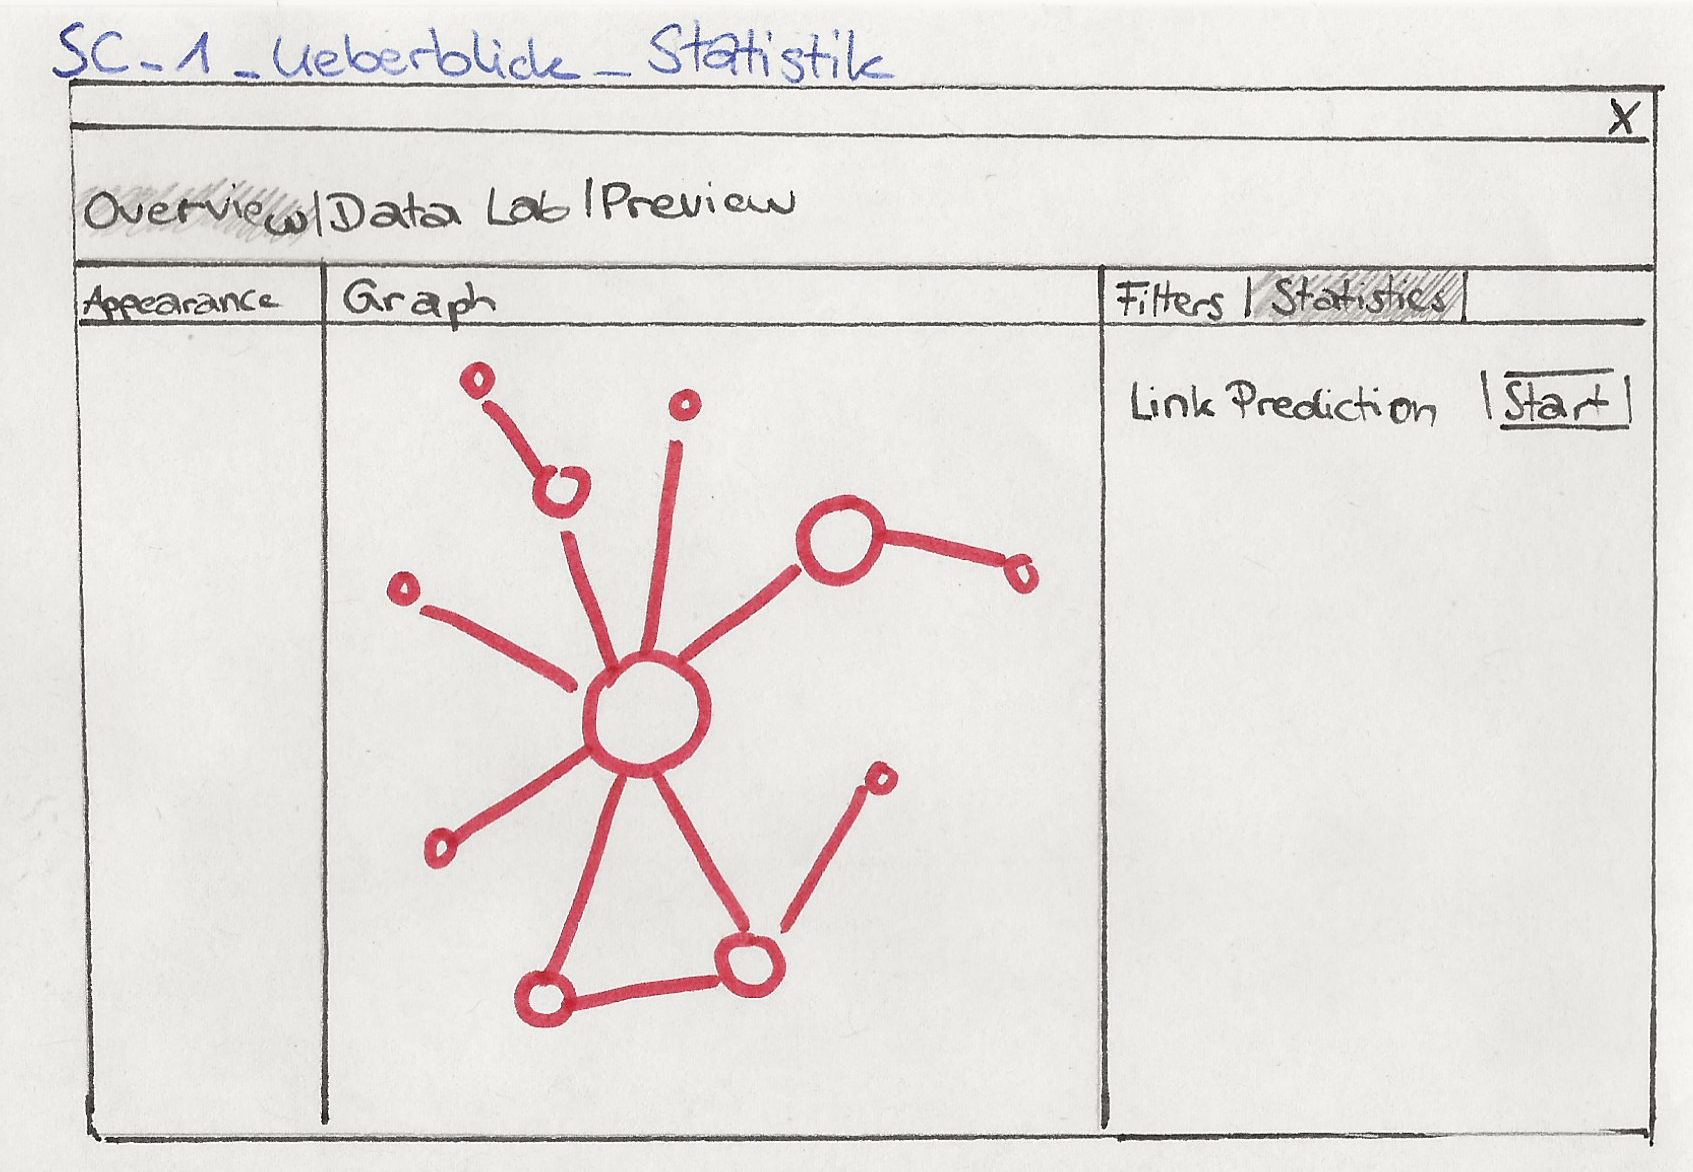
\includegraphics[width=\linewidth]{resources/SC-1.png}
    \caption{Überblick der Ansicht Statistik.}
    \label{fig:screen1}
\end{figure}

Im Bild kann man eine Skizze sehen, welche einen Überblick über den Aufbau von Gephi gibt. Grau hinterlegt sind die
angewählten Menü-Punkte. Unter dem Menü \textit{Statistics} wird hier nun ein Punkt "Link Prediction" mit einem
Start-Button eingefügt. In der Darstellung ausgelassen wurden die anderen Punkte, die bereits in diesem Menü existieren
wie beispielsweise "Average Degree".

\begin{figure}[htbp]
    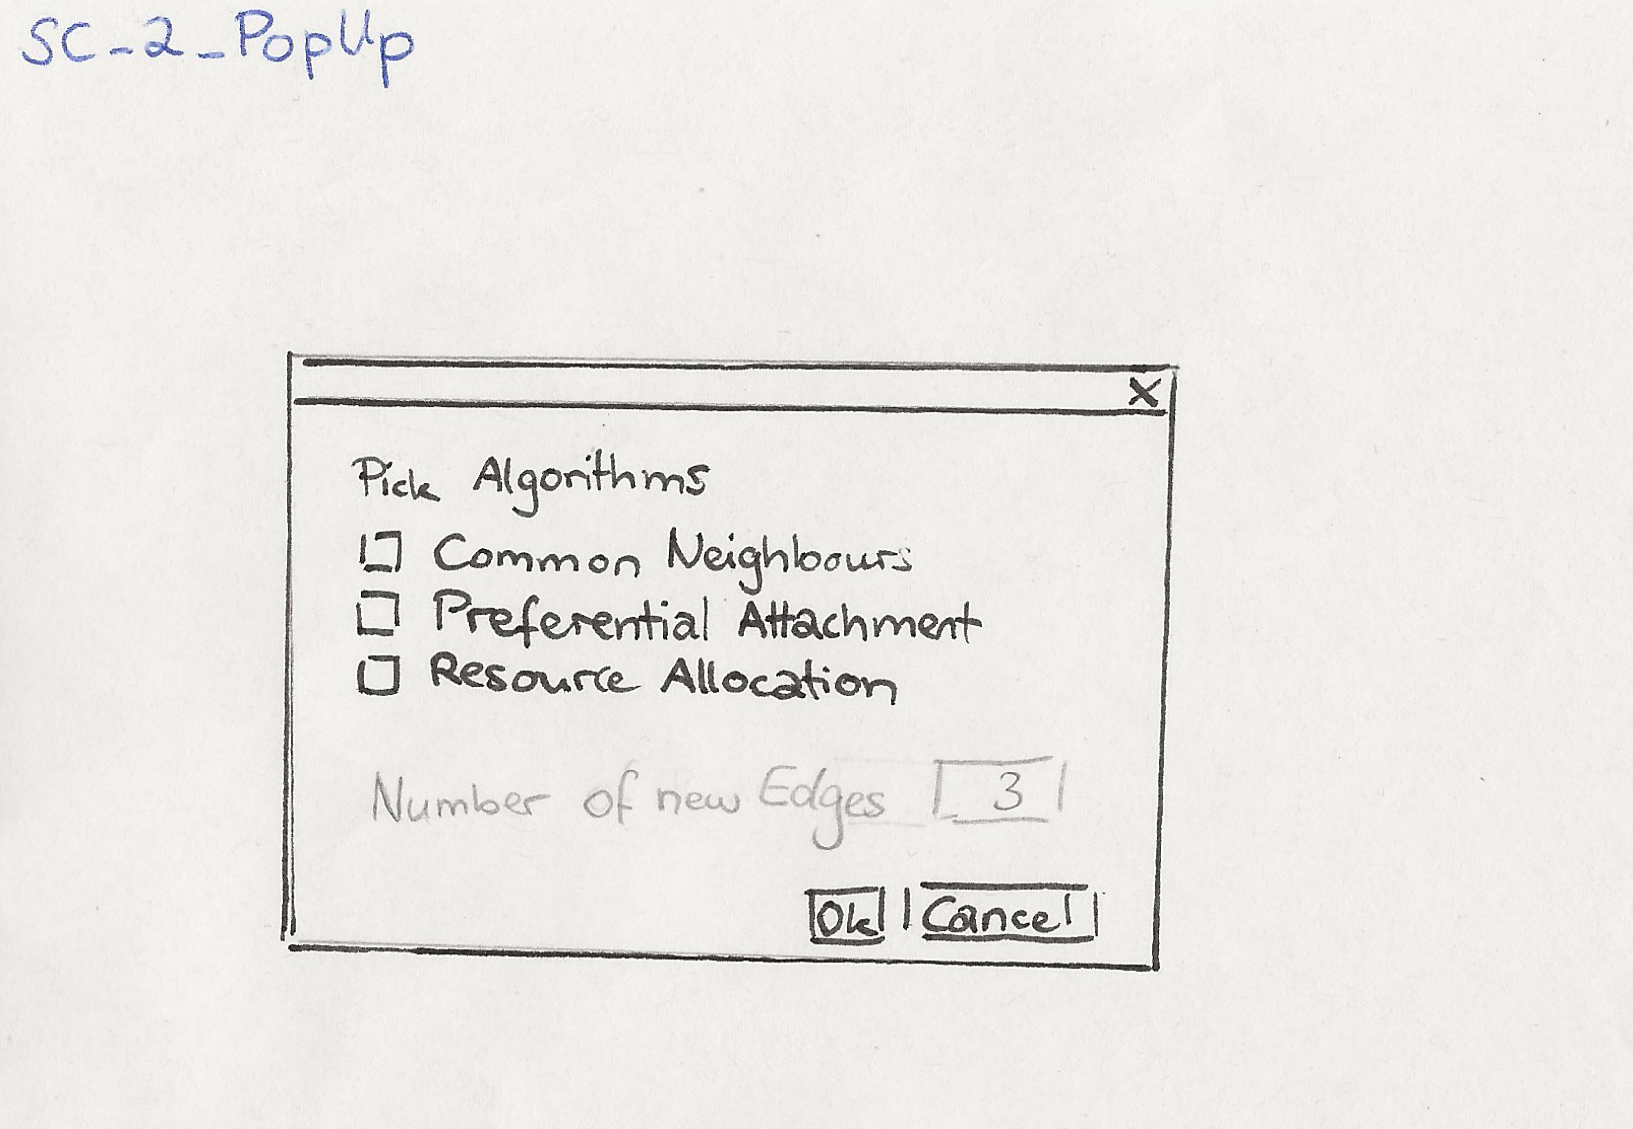
\includegraphics[width=\linewidth]{resources/SC-2.png}
    \caption{Pop-Up für die Auswahl der Berechnung.}
    \label{fig:screen2}
\end{figure}

Hier kann man sehen, dass beim Drücken auf "Start" ein Pop-Up geöffnet wird, in welchem man alle Algorithmen auswählen
kann, für welche die Link Prediction durchgeführt werden soll. In einem zusätzlichen Eingabefeld kann man einen Wert
von 1 bis x eingeben. Dieser besagt, wie viele Durchgänge bei der Link Prediction gemacht werden sollen - also wie viele
neue Kanten dem Graphen hinzugefügt werden.

Die Funktion der zusätzlichen Konfiguration eines Algorithmus ("advanced" Button) wird offen gehalten, wird aber für die
Implementierung des Common Neighbour und Preferential Attachment Algorithmus derzeit nicht benötigt.

Bei einer zu hohen Zahl oder der Auswahl bestimmter langwieriger Algorithmen soll eine Warnung an den User ausgegeben
werden. Wird diese bestätigt, so wird der Algorithmus trotzdem berechnet. Beim Abbruch kann der User seine gewünschten
Einstellungen verändern.

\begin{figure}[htbp]
    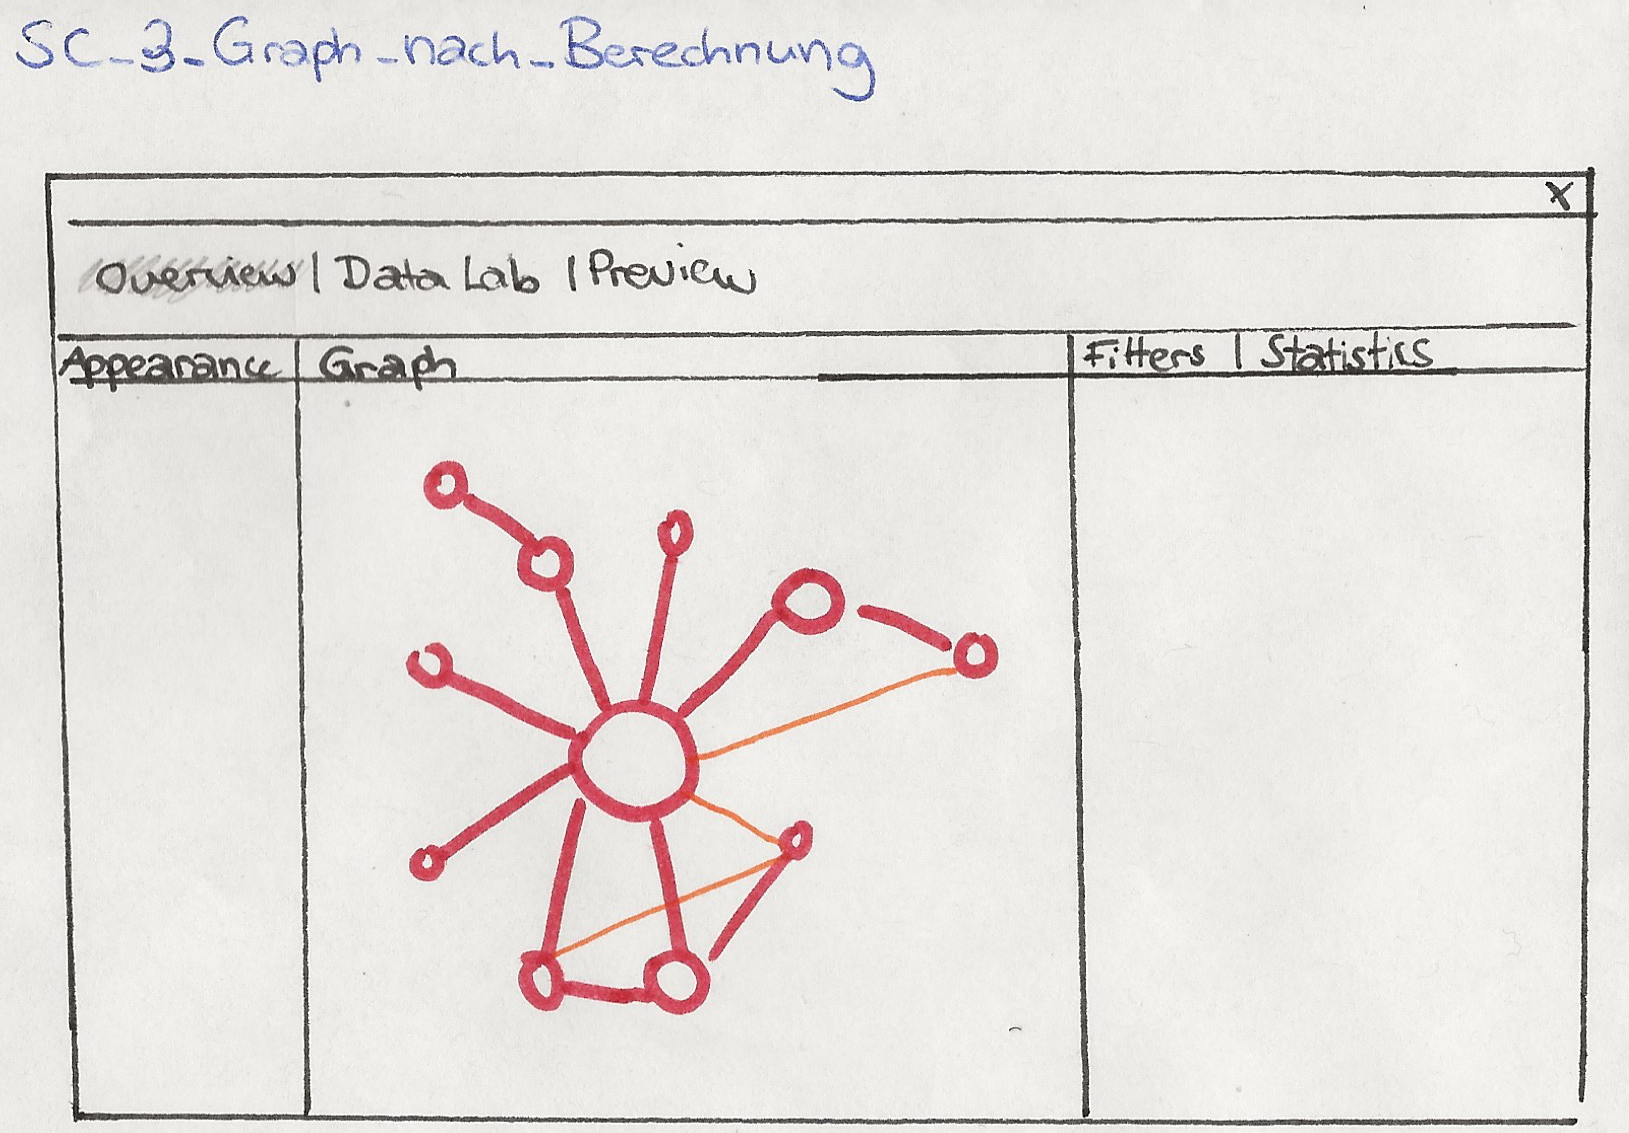
\includegraphics[width=\linewidth]{resources/SC-3.png}
    \caption{Modifizierter Graph mit vorhergesagtem Edge.}
    \label{fig:screen3}
\end{figure}

Im dritten Screen ist der Graph nach der Berechnung zu sehen. Es würden neue Kanten hinzugefügt. Diese können mit Hilfe
der Appearance Einstellungen eingefärbt werden, da im Data Laboratory Felder enthalten sind, die aussagen, ob eine
Kante mit einem Link Prediction Algorithmus hinzugefügt wurde oder ob sie bereits existiert hat.

\begin{figure}[htbp]
    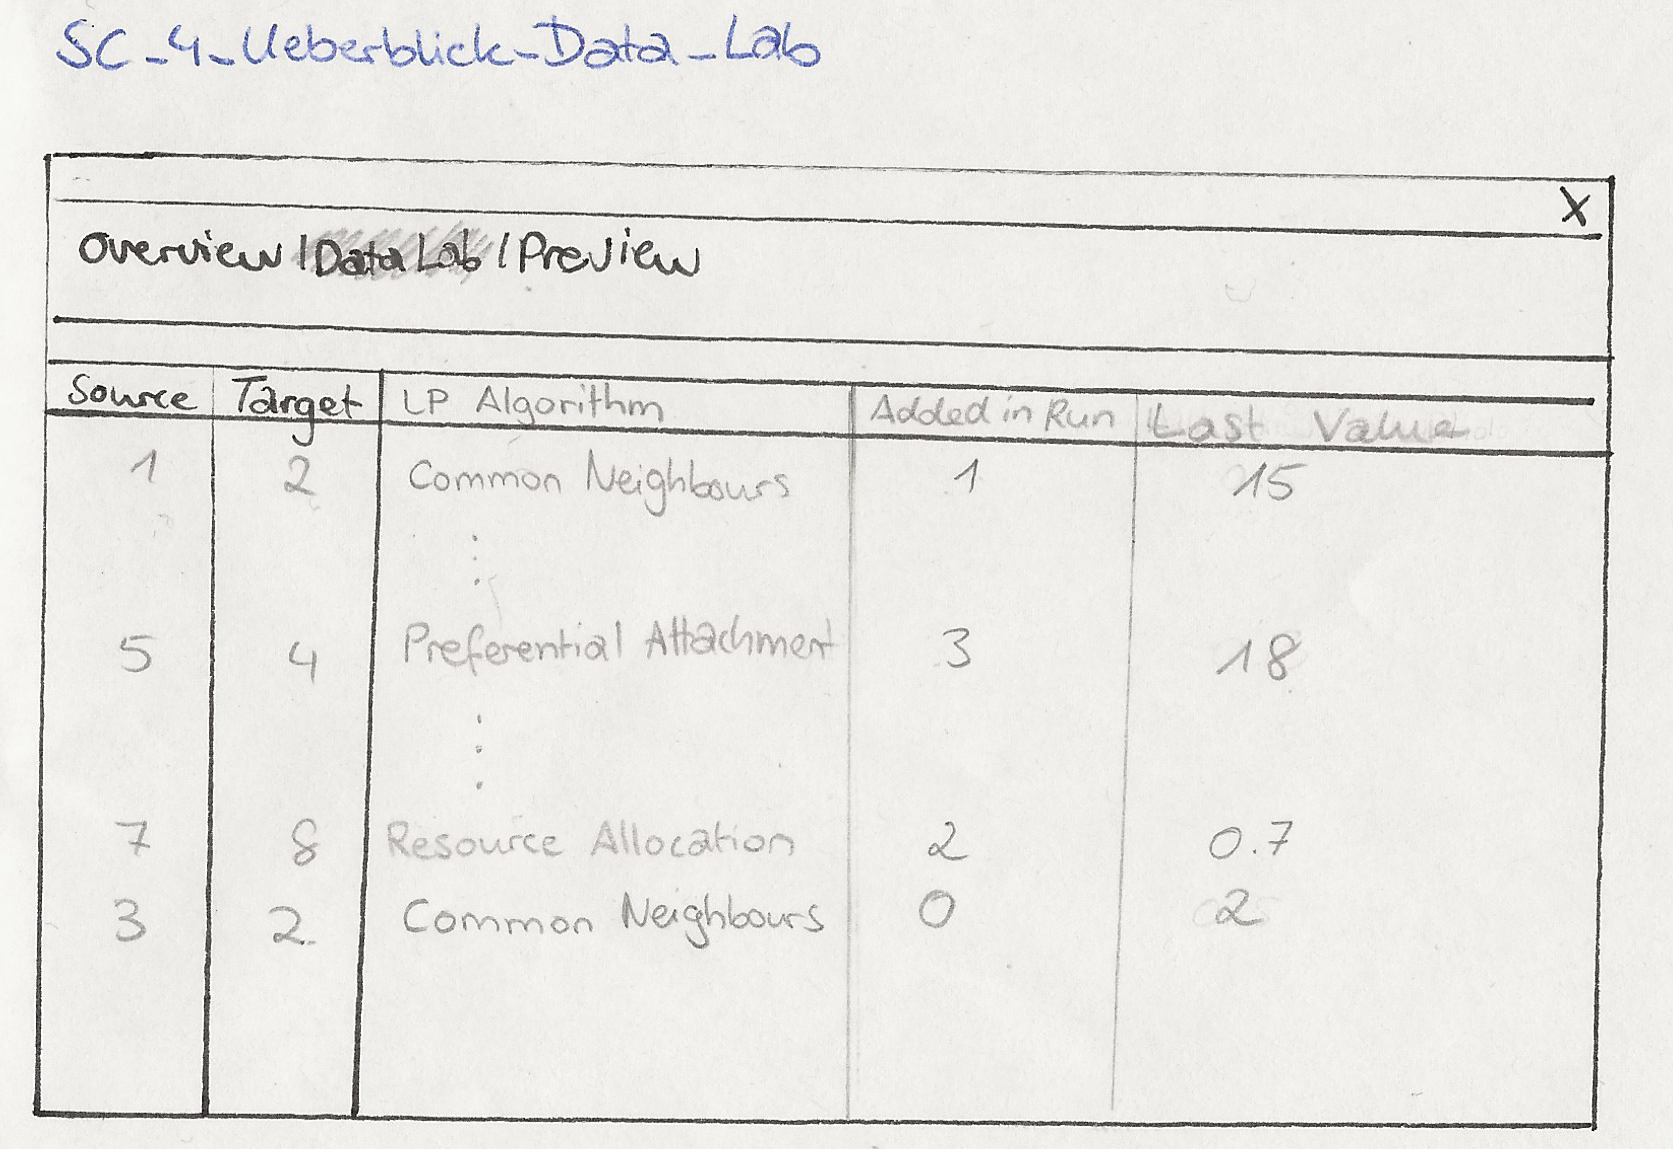
\includegraphics[width=\linewidth]{resources/SC-4.png}
    \caption{Data Laboratory mit neuen Edges.}
    \label{fig:screen4}
\end{figure}

In diesem Bild kann man die durch die Algorithmen neu hinzugefügten Attribute im Data Laboratory sehen. Diese sind auf
den Kanten des Graphen zu finden. Dort gibt es ein Feld "Link Prediction Algorithm", in welchem ein Wert enthalten ist,
um eindeutig zu zeigen, mit welchem Algorithmus diese Kante hinzugefügt wurde.

Eine weitere Spalte ist "Added in Run". Gibt der User bei der Berechnung den Wert 3 mit, so werden hier 3 Kanten pro
ausgewähltem Algorithmus durchnummeriert hinzugefügt. Damit der User einen Überblick hat, in welchem Durchlauf diese
Kante hinzugefügt wurde, haben wir dieses Attribut hinzugefügt. 1 würde dabei für die am wahrscheinlichsten hinzugefügte
Kante im ersten Durchlauf stehen, 3 für die wahrscheinlichste im dritten Durchlauf, usw.

Bei Kanten, die bereits vorhanden sind, werden Default Werte für die Spalten "Link Prediction Algorithmus" und "Added
in Run" eingefügt.

Die letzte Spalte "Last Threshold Link Prediction" ist eine optionale Spalte, bei der wir noch weitere Analysen
durchführen müssen, um zu evaluieren, ob diese einen tieferen Sinn hat. Hier würde zum Beispiel der letzte berechnete
Wert einer neu hinzugefügten Kante eingetragen werden. Dann wäre diese im Fall von keiner Berechnung, da die Kante
bereits existierte, ebenfalls mit einem Default-Wert befüllt.

\subsection{Filtern der neuen Link Prediction Kanten}

Die neu errechneten Link Prediction Werte sollen gefiltert werden können. Auch dazu wurden einige Skizzen erstellt.

\begin{figure}[htbp]
    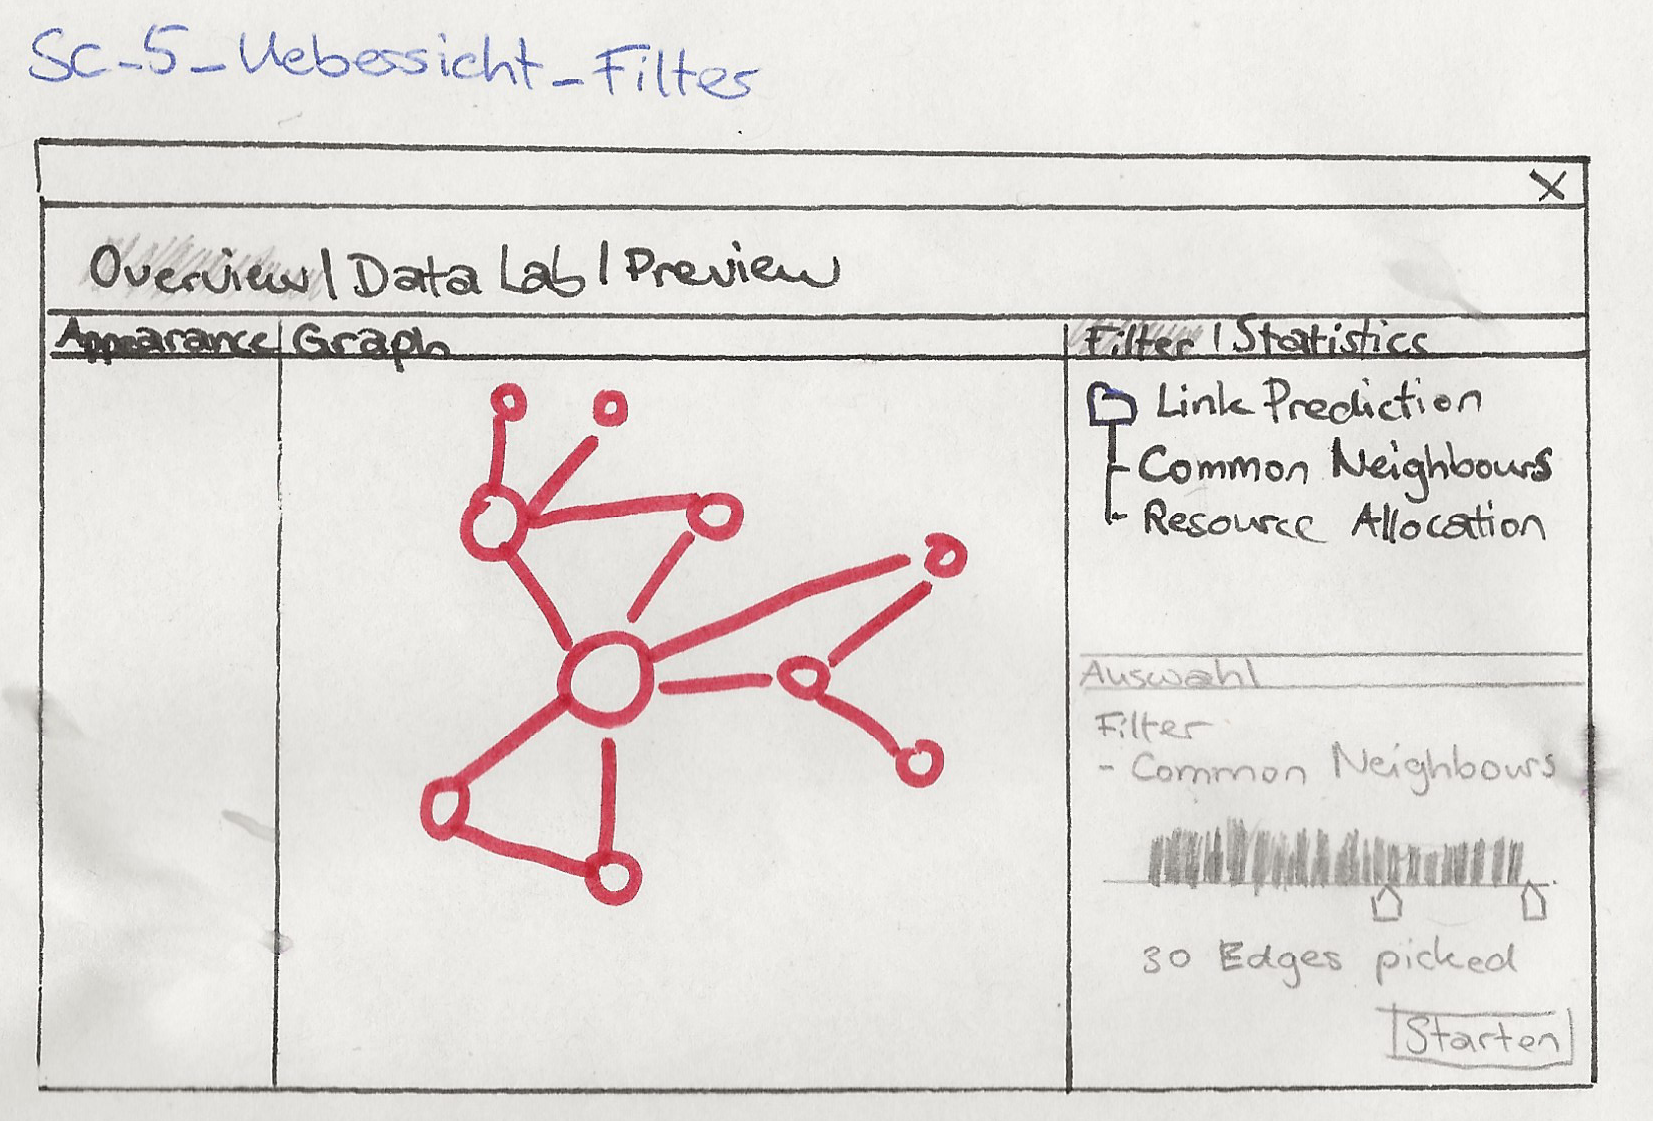
\includegraphics[width=\linewidth]{resources/SC-5.png}
    \caption{Überblick der Ansicht Filter.}
    \label{fig:screen5}
\end{figure}

Im Überblick ist zu sehen, wie der Link Prediction Filter in das bestehende GUI eingebunden wird. Dort wird es unter
\textit{Filter} einen neuen Ordner "Link Prediction" geben. Unter diesem können die Filter für einzelne Algorithmen
angewählt werden. Danach kann eingestellt werden, welche Links von welchen Durchläufen angezeigt werden sollen. Wird auf
"Start" geklickt, wird allenfalls das folgende Pop-Up angezeigt:

\begin{figure}[htbp]
    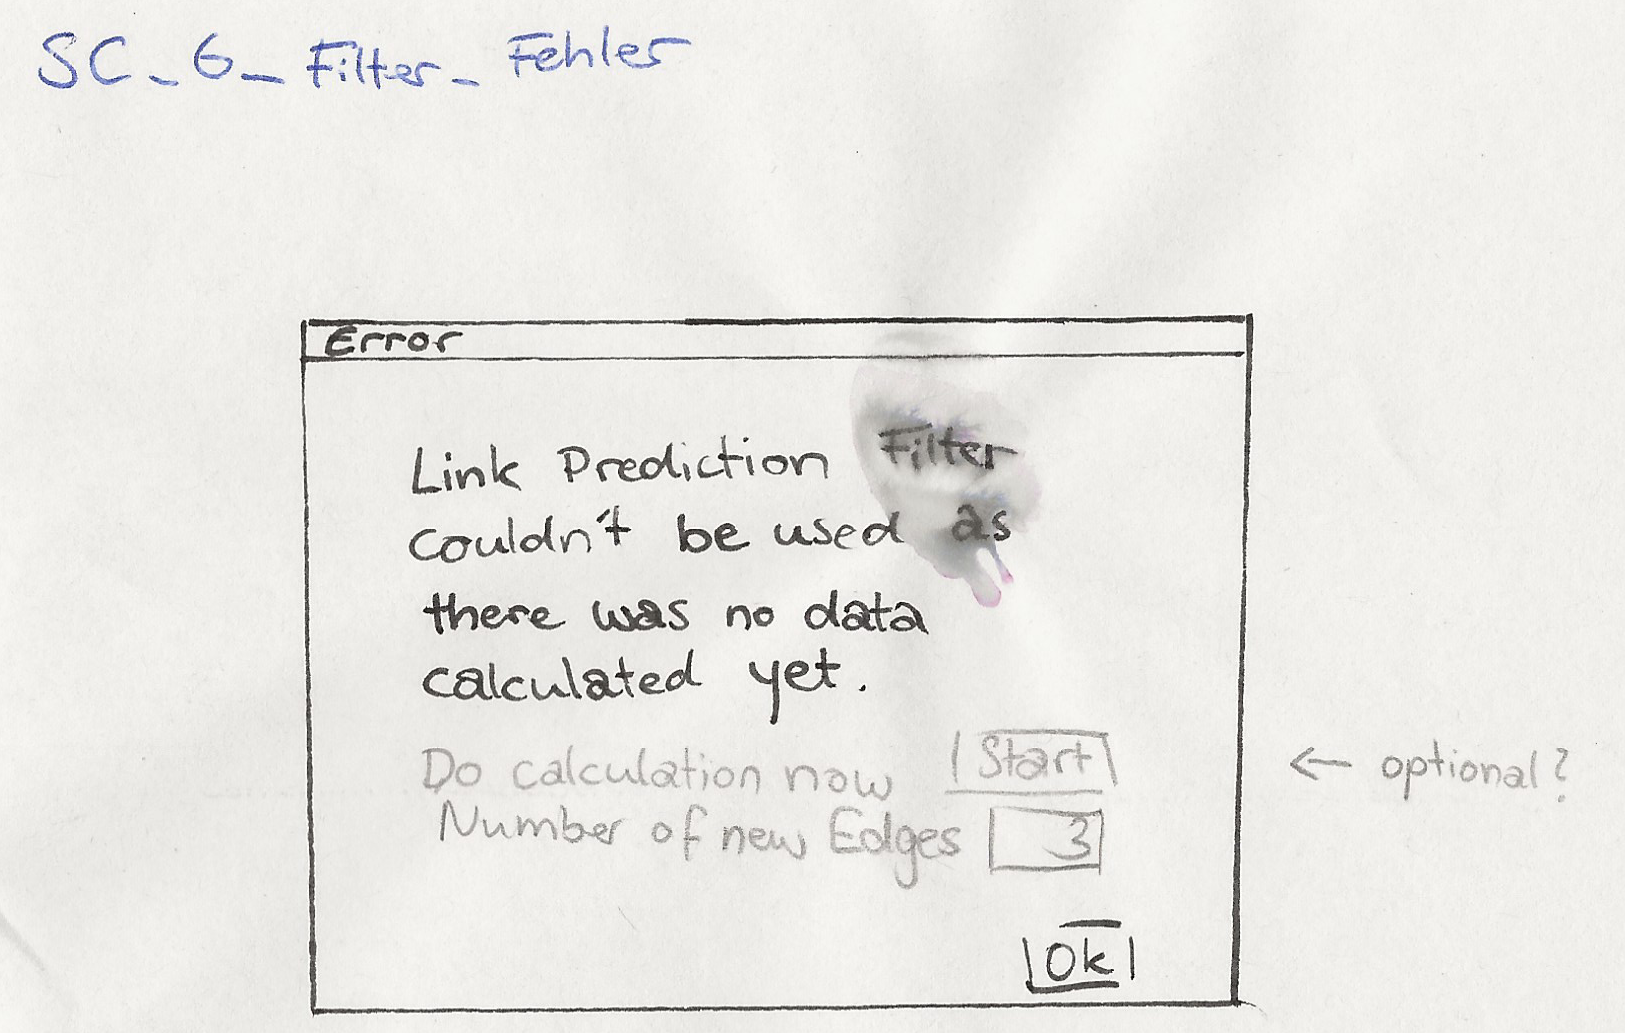
\includegraphics[width=\linewidth]{resources/SC-6.png}
    \caption{Fehlermeldung, wenn die Berechnung der Link Prediction noch nicht durchgeführt wurde.}
    \label{fig:screen6}
\end{figure}

Dieses Pop-Up stellt eine Fehlermeldung dar. Dort wird anstelle von "Link Prediction Filter" der ausgewählte Filter
stehen beispielsweise "Common Neighbour Filter" stehen. Diese Fehlermeldung erscheint, sofern die Berechnungen, um den
Filter anzuwenden, noch nicht ausgeführt wurden.

Optional behält sich das Projektteam vor, eine Option einzubauen, bei der direkt aus dem Fenster der Fehlermeldung die
Berechnung für diesen speziellen Algorithmus gestartet werden kann. Andernfalls kann die Fehlermeldung weggeklickt
werden und dann über die \textit{Statistics} die Berechnung vorgenommen werden.

\begin{figure}[htbp]
    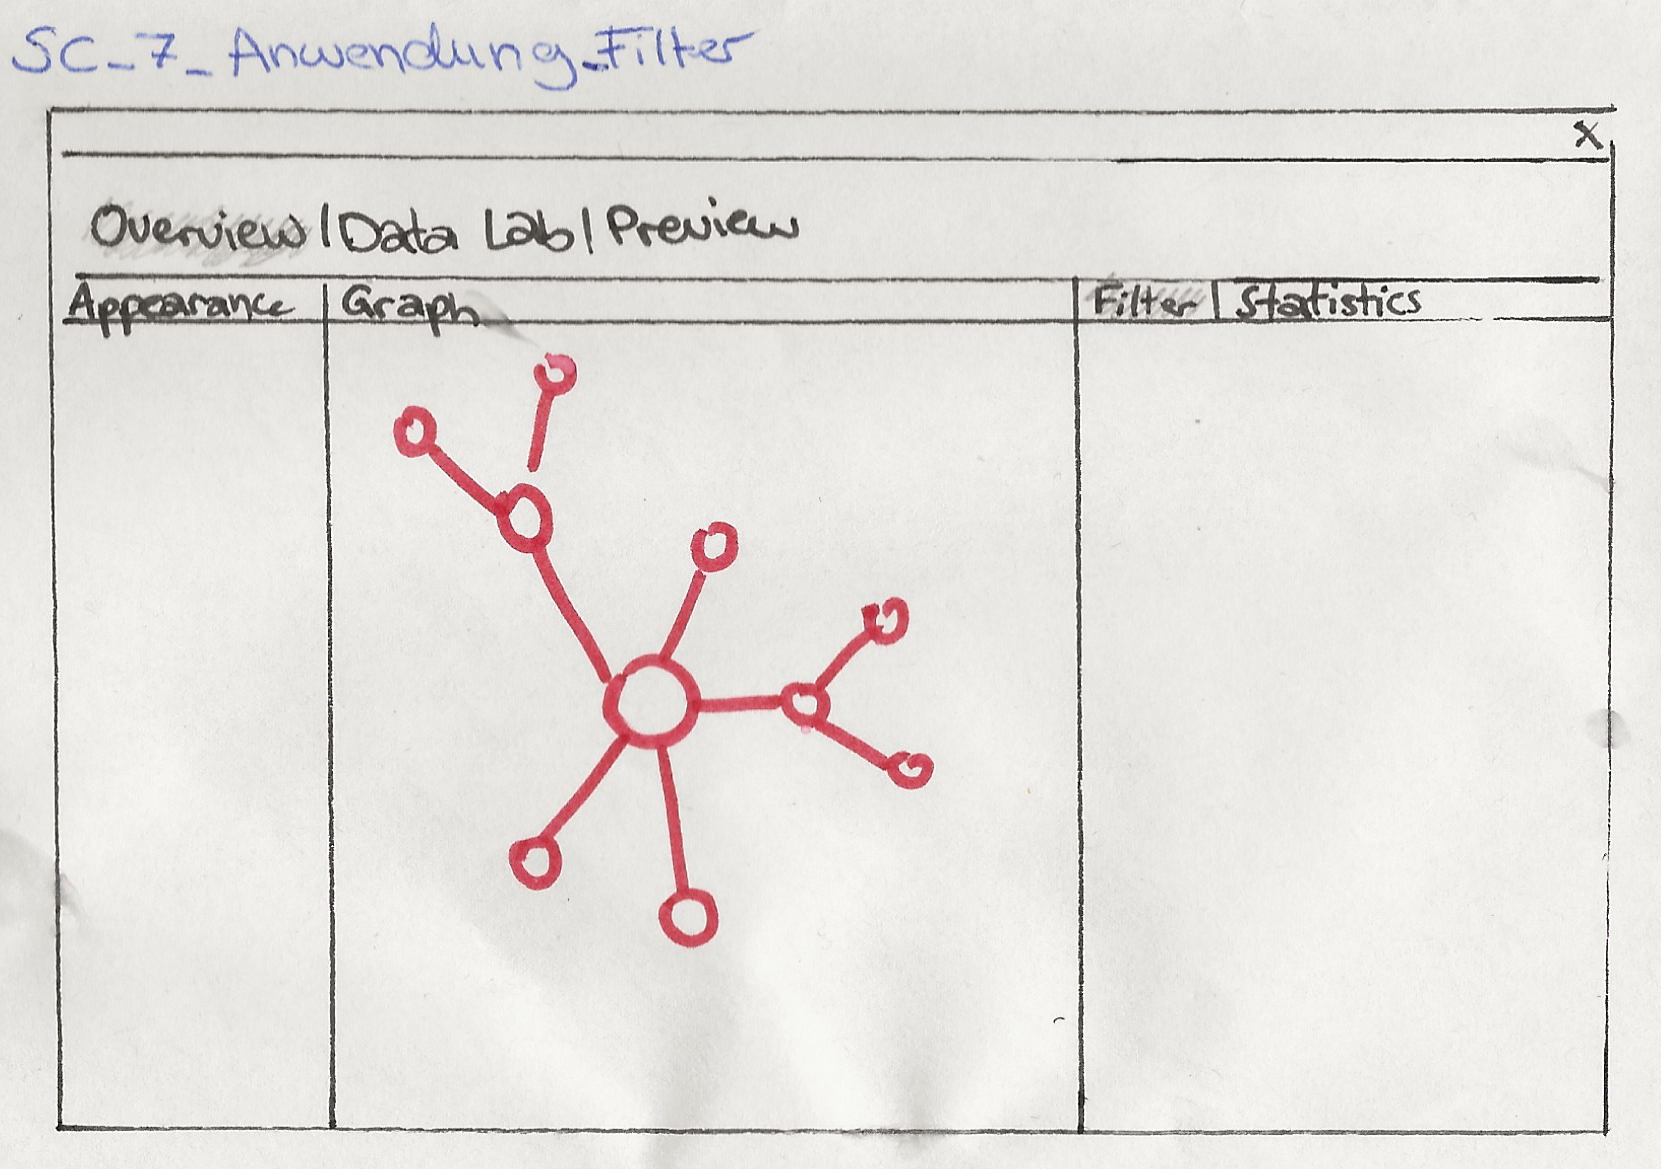
\includegraphics[width=\linewidth]{resources/SC-7.png}
    \caption{Gefilterter Graph.}
    \label{fig:screen7}
\end{figure}

Wurde der Filter angewendet, so wird der Graph dargestellt mit den neu ergänzten Kanten. Die bereits vor der Berechnung
eingefügten Kanten werden auch dann angezeigt, egal wie hier gefiltert wird.

\subsection{Vergleich der Link Prediction Algorithmen mit tatsächlichen neuen Links}

Dummy text.

\section{Link Prediction}

\subsection{Algorithmen (allgemein)}

Nach Recherche über die verschiedenen Algorithmen wurde entschieden, die Algorithmen "Common Neighbours" und
"Preferential Attachment" zu implementieren. Diese Entscheidung beruhte darauf, dass sich die beiden Algorithmen
insofern unterscheiden, dass beim Common-Neighbours-Algorithmus nur Knoten eine Rolle spielen, welche gemeinsame
Nachbarn aufweisen. Beim zweiten Algorithmus ist dies anders: Dort werden alle Knoten im Bezug aufeinander
berücksichtigt - hier ist also die Popularität eines einzelnen entscheidend, während beim ersteren Gemeinsamkeiten im
Vordergrund stehen.

Ausserdem wurde festgelegt, dass man sich in dieser Arbeit darauf beschränkt, die ungerichteten Graphen anzuschauen.
Die gewöhnlichen Algorithmen sind nicht spezifisch anwendbar auf gerichtete Graphen, so dass im Rahmen dieser Arbeit
auch diese als ungerichtet betrachtet werden. Eine Anmerkung diesbezüglich soll es bei der Link Prediction in Gephi
dementsprechend auch geben.

Die Begründung für diese Entscheidung beruht darauf, dass die Algorithmen, welche für gerichtete Graphen derzeit
entwickelt wurden, eine wesentlich höhere Komplexität aufweisen. Dies hätte dann einen Einfluss auf den vom Kunden
gewünschten Projektumfang - eventuell hätten dann Abstriche beim zweiten Teil des Projekts gemacht werden müssen.

\subsection{Algorithmus: Common Neighbours}

Dummy text.

\subsection{Algorithmus: Preferential Attachment}

Dummy text.

\section{Netzwerk- und Algorithmenvergleich}

Dummy text.
\chapter{Diskussion und Ausblick}

Das Erarbeiten des Link-Prediction-Plugins war eine herausfordernde und zugleich lehrreiche Arbeit.
Mit dem Projekt einher ging die Möglichkeit, im Open-Source-Umfeld zu einer etablierten Software beizutragen.
Insesondere das modulübergreifende Anwenden von Wissen aus dem Studiengang und der Austausch im Team und mit dem Betreuer bereitete grosse Freude.
In den folgenden Kapiteln werden die Resultate reflektiert und ein Ausblick auf nacholgende Tätigkeiten dargeboten.

\section{Erreichtes}

Das Ziel, ein Link-Prediction-Plugin zu entwickeln, ist erreicht worden.
Neben den erforderlichen Funktionen zur Vorhersage von Links und zur Evaluation der verschiedenen Algorithmen wurde zusätzlich ein Filter zum selektieren der Kanten je Algorithmus entwickelt.
Die verwendete Architektur erlaubt es, einfach neue Link-Prediction-Algorithmen und Kennzahlen zur Beurteilung der Qualität der Algorithmen hinzuzufügen.
Als Reaktion auf die anfänglich langen Laufzeiten bei grossen Graphen wurde die Berechnung der Link-Predictions optimiert:
Für die Berechnung der Link-Prediction-Werte müssen sämtliche Knoten initial zweimal durchlaufen werden.
Indem beim Hinzufügen einer neuen Kante nur die beiden davon betroffenen Kanten geändert werden, kann der Aufwand für alle weiteren Iterationen drastisch reduziert werden.

Tests mit der aktuellen Implementierung haben gezeigt, das Link-Predictions in Graphen mit bis zu 1000 Knoten problemlos berechnet werden können.
Das Berechnen in grösseren Graphen kann in längeren Laufzeiten resultieren.
Ein entsprechender Hinweis wurde im README.md vermerkt.

\section{Ausblick}

Trotz diverser Optimierungsbemühungen müssen beim initialien Berechnen der Prediction-Werte alle Knoten zweimal durchlaufen werden.
Dies erfordert bei grossen Netzwerken seine Zeit.
Um auch bei solchen Netzwerken eine schnellere Performance zu erreichen, müssten weitere Optimierungsmassnahmen in Betracht gezogen werden.
Folgende Möglichkeiten würden sich dazu anbieten:

\begin{itemize}
    \item Anstatt, dass die Vorhersagen für alle Knoten berechnet werden, könnte man im \acs{ui} die Möglichkeit anbieten, ein Subset bestehend aus spezifischen Knoten auszuwählen. Damit würde die Berechnung nur für alle relevanten Knoten durchgeführt.
    \item Falls ein Clustering zur Verfügung steht (entweder über ein Knoten-Attribut oder über eine berechnete Messgrösse), könnte man die Berechnung auf alle Knoten dieses Clusters beschränken.
    \item Die Berechnung der verschiedenen Algorithmen könnte parallelisiert durchgeführt werden. Aktuell wird der Graph während der Berechnung mit einem Write-Lock geschützt. Dieser müsste für die Parallelisierung unter Berücksichtigung allfälliger Nebeneffekte aufgehoben werden.
\end{itemize}

Aktuell werden vom Plugin nur ungerichtete und ungewichtete Graphen unterstützt.
Falls die Algorithmen auf gerichtete Graphen angewendet werden, werden ausgehende und eingehende Kanten zwischen denselben zwei Knoten als eine Kante betrachtet:
Ein Graph mit einer Kante von Knoten $A$ nach Knoten $C$ und einer Kante von Knoten $C$ nach Knoten $A$ würde von den Algorithmen als eine Kante zwischen den beiden Knoten interpretiert.
In künftigen Releasen könnte zusätzlich die Funktionalität angeboten werden, ungerichtete und gerichtete Graphen unterschiedlich zu behandeln.

Weiter könnten auch Kantengewichte mit in die Berechnungen einbezogen werden.
Aktuell werden diese ignoriert und neue Kanten nicht gewichtet.
% TODO Verweis auf Literatur für Algorithmen mit gewichteten Kanten


\backmatter


\listoffigures

\bibliographystyle{plain}
\bibliography{refs}

\chapter*{Glossar}

\begin{acronym}
    %TODO: Pfad, Knoten, Kante
    \acro{avgsp}[Average Shortest Path]{Durchschnittliche Länge des kürzesten Pfads zwischen zwei Knoten i und j.}
    \acro{clique}[Clique]{Subgraph innerhalb eines Graphen, in welchem die Knoten untereinander stark verbunden sind.}
    \acro{cc}[Cluster Coefficient] Messgrösse, welche das Mass der Cliquenbildung in einem Graphen aufzeigt.
    \acro{datalaboratory}[Data Laboratory]{Knoten- und Kantentabellen eines Graphen in Gephi.}
    \acro{density}[Density]{Messgrösse, welche verdeutlicht, wie komplett die Knotten des Netzwerks miteinander verbunden sind.}
    \acro{diameter}[Diameter]{Messgrösse, welche den längsten kürzesten Pfad zwischen allen Knottenpaaren in einem Graphen entspricht.}
    \acro{gephi}[Gephi]{Gephi ist eine Open-Source Software zur explorativen
    Analyse von Graphen. Die Software ist in der Programmiersprache Java implementiert
    und modular aufgebaut.}
\end{acronym}


\appendix
\chapter{Anhang}

\section{Projektvereinbarung}
\label{projektvereinbarung}

\newpage

\section{Proof of Concept}
\label{poc}

Für die Einarbeitung in die Gephi-Plugin Entwicklung und erste Ansätze für die Umsetzung des Projekts zu finden, hat
sich das Projektteam entschlossen, ein Proof of Concept durchzuführen.

\subsection{Ziel}

Mit dem Proof of Concept, soll sich einerseits mit dem \ac{api} von \acs{gephi} vertraut zu machen.
Andererseits soll die Funktionsweise von ersten Ideen und Konzepten überprüft werden.

\subsection{Umsetzungsprozess}

\begin{itemize}
    \item \textbf{Filter:} Filter werden in \acs{gephi} verwendet, um ein Netzwerk auf Knoten oder Kanten zu reduzieren, welche bestimmte Eigenschaften besitzen.
    In Bezug auf Link-Prediction wurde deshalb eine neue Filterkategorie eingeführt, unter welcher nach verschiedenen Prediction-Algorithmen gefiltert werden kann.
    Durch Auswahl eines Algorithmus können jene Kanten herausgefiltert werden, welche durch Anwenden des Algorithmus neu hinzugefügt werden.
    Der Filter wird dabei um ein \acs{ui}-Element ergänzt, bei welchem die Anzahl der hinzugefügten Kanten eingegrenzt werden kann.

    \item \textbf{Statistiken:} Die Wahrscheinlinkteit, dass sich eine neue Kante zwischen zwei Knoten bildet, entspricht einem berechneten Wert.
    Diese Berechnung wird mittels Statistiken angestossen. Die gesamte Logik und Berechnung der verschiedenen Algorithmen wird anschliessend
    durch verschiedene Statistik-Objekte gekapselt.

    Die Funktionsweise für das Implementieren von neuen Statistik-Objekten ist im Gephi-Plugin Bootcamp gut dokumentiert. Darauf aufbauend
    konnte ein neues Statistik-Objekt mit entstprechendem Button im \acs{ui} implementiert werden. Bei der Berechnung wurde der Algorithmsu
    ``Common Neighbours'' eingesetzt, bei welchem die Anzahl Nachbarn jedes Knotens gezählt werden.

    Für die Implementierung des Algorithmus konnten bestehende Funktionen von \acs{gephi} verwendet werden um die Knoten aus dem Graphen, respektive
    dessen Nachbarn auszulesen. Die berechneten Werte konnten anschliessend bereits im \acs{datalaboratory} abgelegt werden.

    % TODO: Redundant?
    %Da für die Umsetzung der Link Prediction aber nicht nur die direkte Anzahl der Nachbarn relevant ist, sondern vor allem
    %die Zahl der gemeinsamen Nachbarn zweier Knoten wurde auch dafür noch eine Statistik umgesetzt. Hier werden nacheinander
    %die Knoten durchgegangen und getestet, wie viele ihrer Nachbarn mit den Nachbarn eines anderen Knotens übereinstimmen.
    %Wenn es noch keine Kante zwischen den beiden Knoten gibt, wird eine neue hinzugefügt und die Anzahl der gemeinsamen
    %Knoten als neues Attribut eingefügt. Wenn es die Kante bereits gibt, wird nur das neue Attribut befüllt. Zusätzlich
    %gibt es ein Attriut, das anzeigt, ob die Kante hinzugefügt wurde oder ob sie schon existiert hat. Zur Berechnung der
    %gemeinsamen Nachbarn werden darüber hinaus nur Kanten gewertet, die nicht erst bei der Berechnung hinzugefügt worden
    %sind.

    Damit dem Graphen Kanten hinzugefügt werden können, während diese noch gelesen und überarbeitet werden, muss ein Write-Lock
    verwendet werden. Die Logik, welche für den Algorithmus ``Common Neighbours'' implementiert wurde, kann für die spätere Umsetzung
    grösstenteils wiederverwendet werden.
\end{itemize}

\subsection{Erkenntnisse}

Es konnten verschiedene Erkenntnisse aus der Umsetzung des Proof Of Concept gewonnen werden.
Zum einen war es sehr hilfreich, sich zum ersten Mal aktiv mit dem \acs{api} von \acs{gephi} zu beschäftigen. Besonders wichtig war
dabei die Erkenntnis, dass die Beispiele aus dem Bootcamp teilweise veraltet sind. Um solche Beispiele mit einer neuen \acs{gepi}-Version
und den dadurch unterschiedlichen \acs{API}s zum Laufen zu bringen, muss zusätzlich Aufwand eingerechnet werden.

Weiter konnte mithilfe des Proof Of Concepts sichergestellt werden, dass sämtliche Installationen, Konfigurationen und die
Entwicklungsumgebung korrekt funktionieren. Viele konfigurative Probleme konnten hier bereits erkannt und frühzeitig behoben werden.

Vom technischen Aspekt her konnten wichtige Erkenntnisse für die spätere Umsetzung gewonnen werden - beispielsweise
wie ein Gephi-Plugin aufgebaut ist. Diese Erkenntnisse fliessen direkt in die Überlegungen beim Entwurf der Software-Architektur ein.
% TODO: Redundant?
%Um ein Beispiel zu nennen, konnte nach der Umsetzung des
%Proof of Concept aber bereits festgelegt werden, wie sichergestellt werden kann, dass die Anzahl Algorithmen für die
%Link Prediction beliebig erweitert werden kann, nämlich indem diverse Informationen in separate Klassen ausgelagert
%werden und es für jeden Algorithmus eine eigene Subklasse gibt, die grundsätzlich nur noch die Umsetzung des Algorithmus
%implementiert, jedoch nichts mit dessen Aufruf zu tun hat.
\newpage

\section{README.md}
\label{readme}

% Split readme in 3 parts
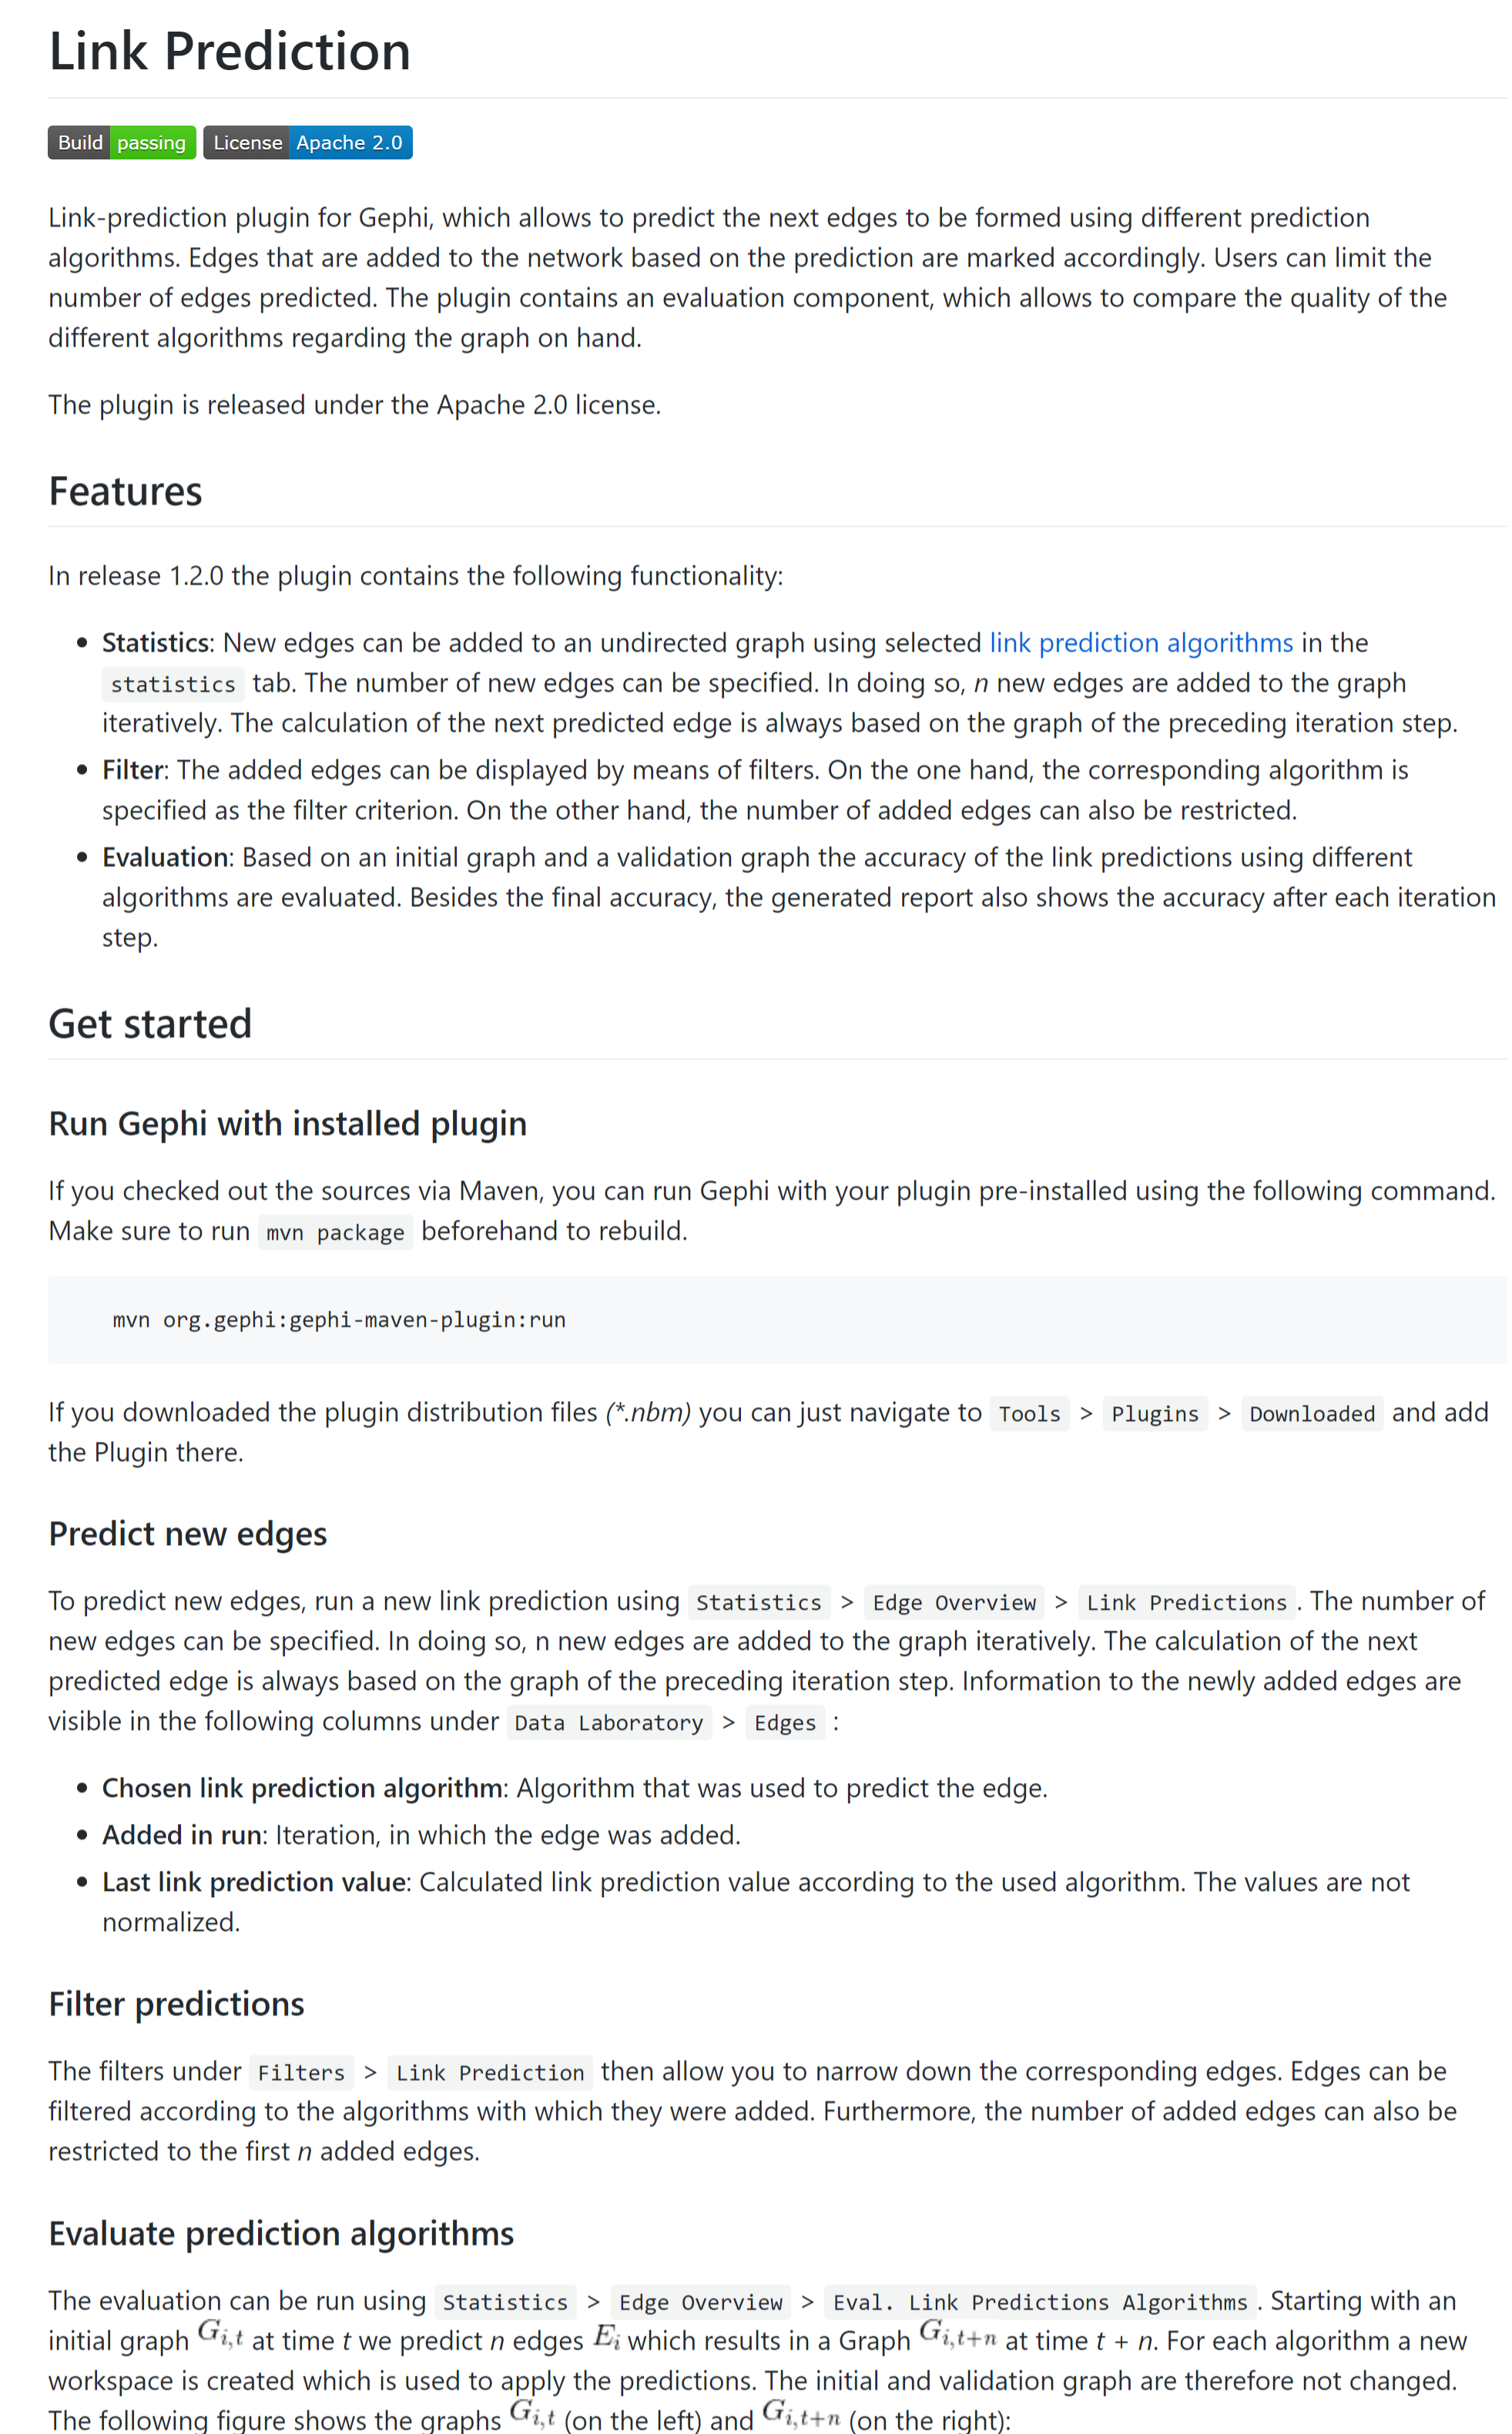
\includegraphics[width=\textwidth]{resources/readme_pt1.png}
\newpage
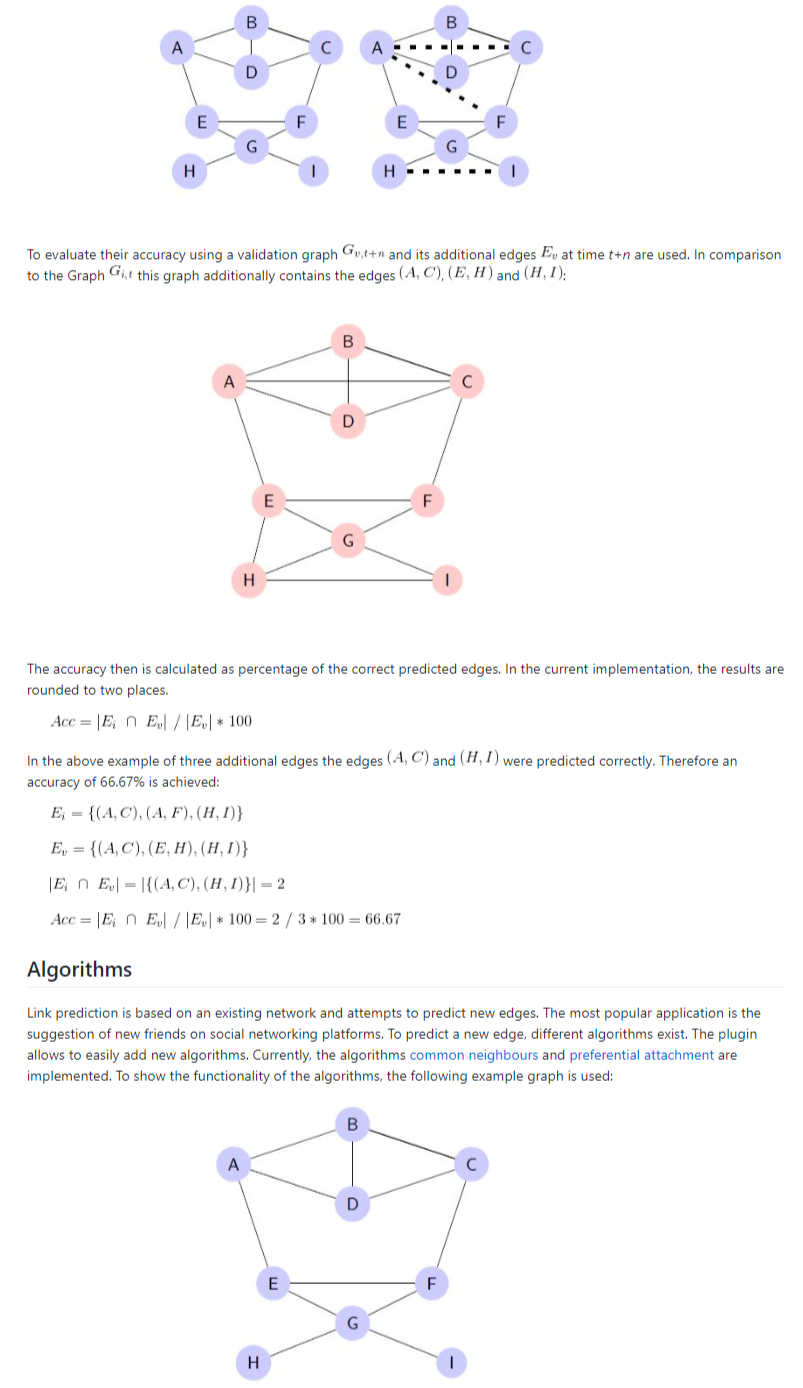
\includegraphics[width=\textwidth]{resources/readme_pt2.png}
\newpage
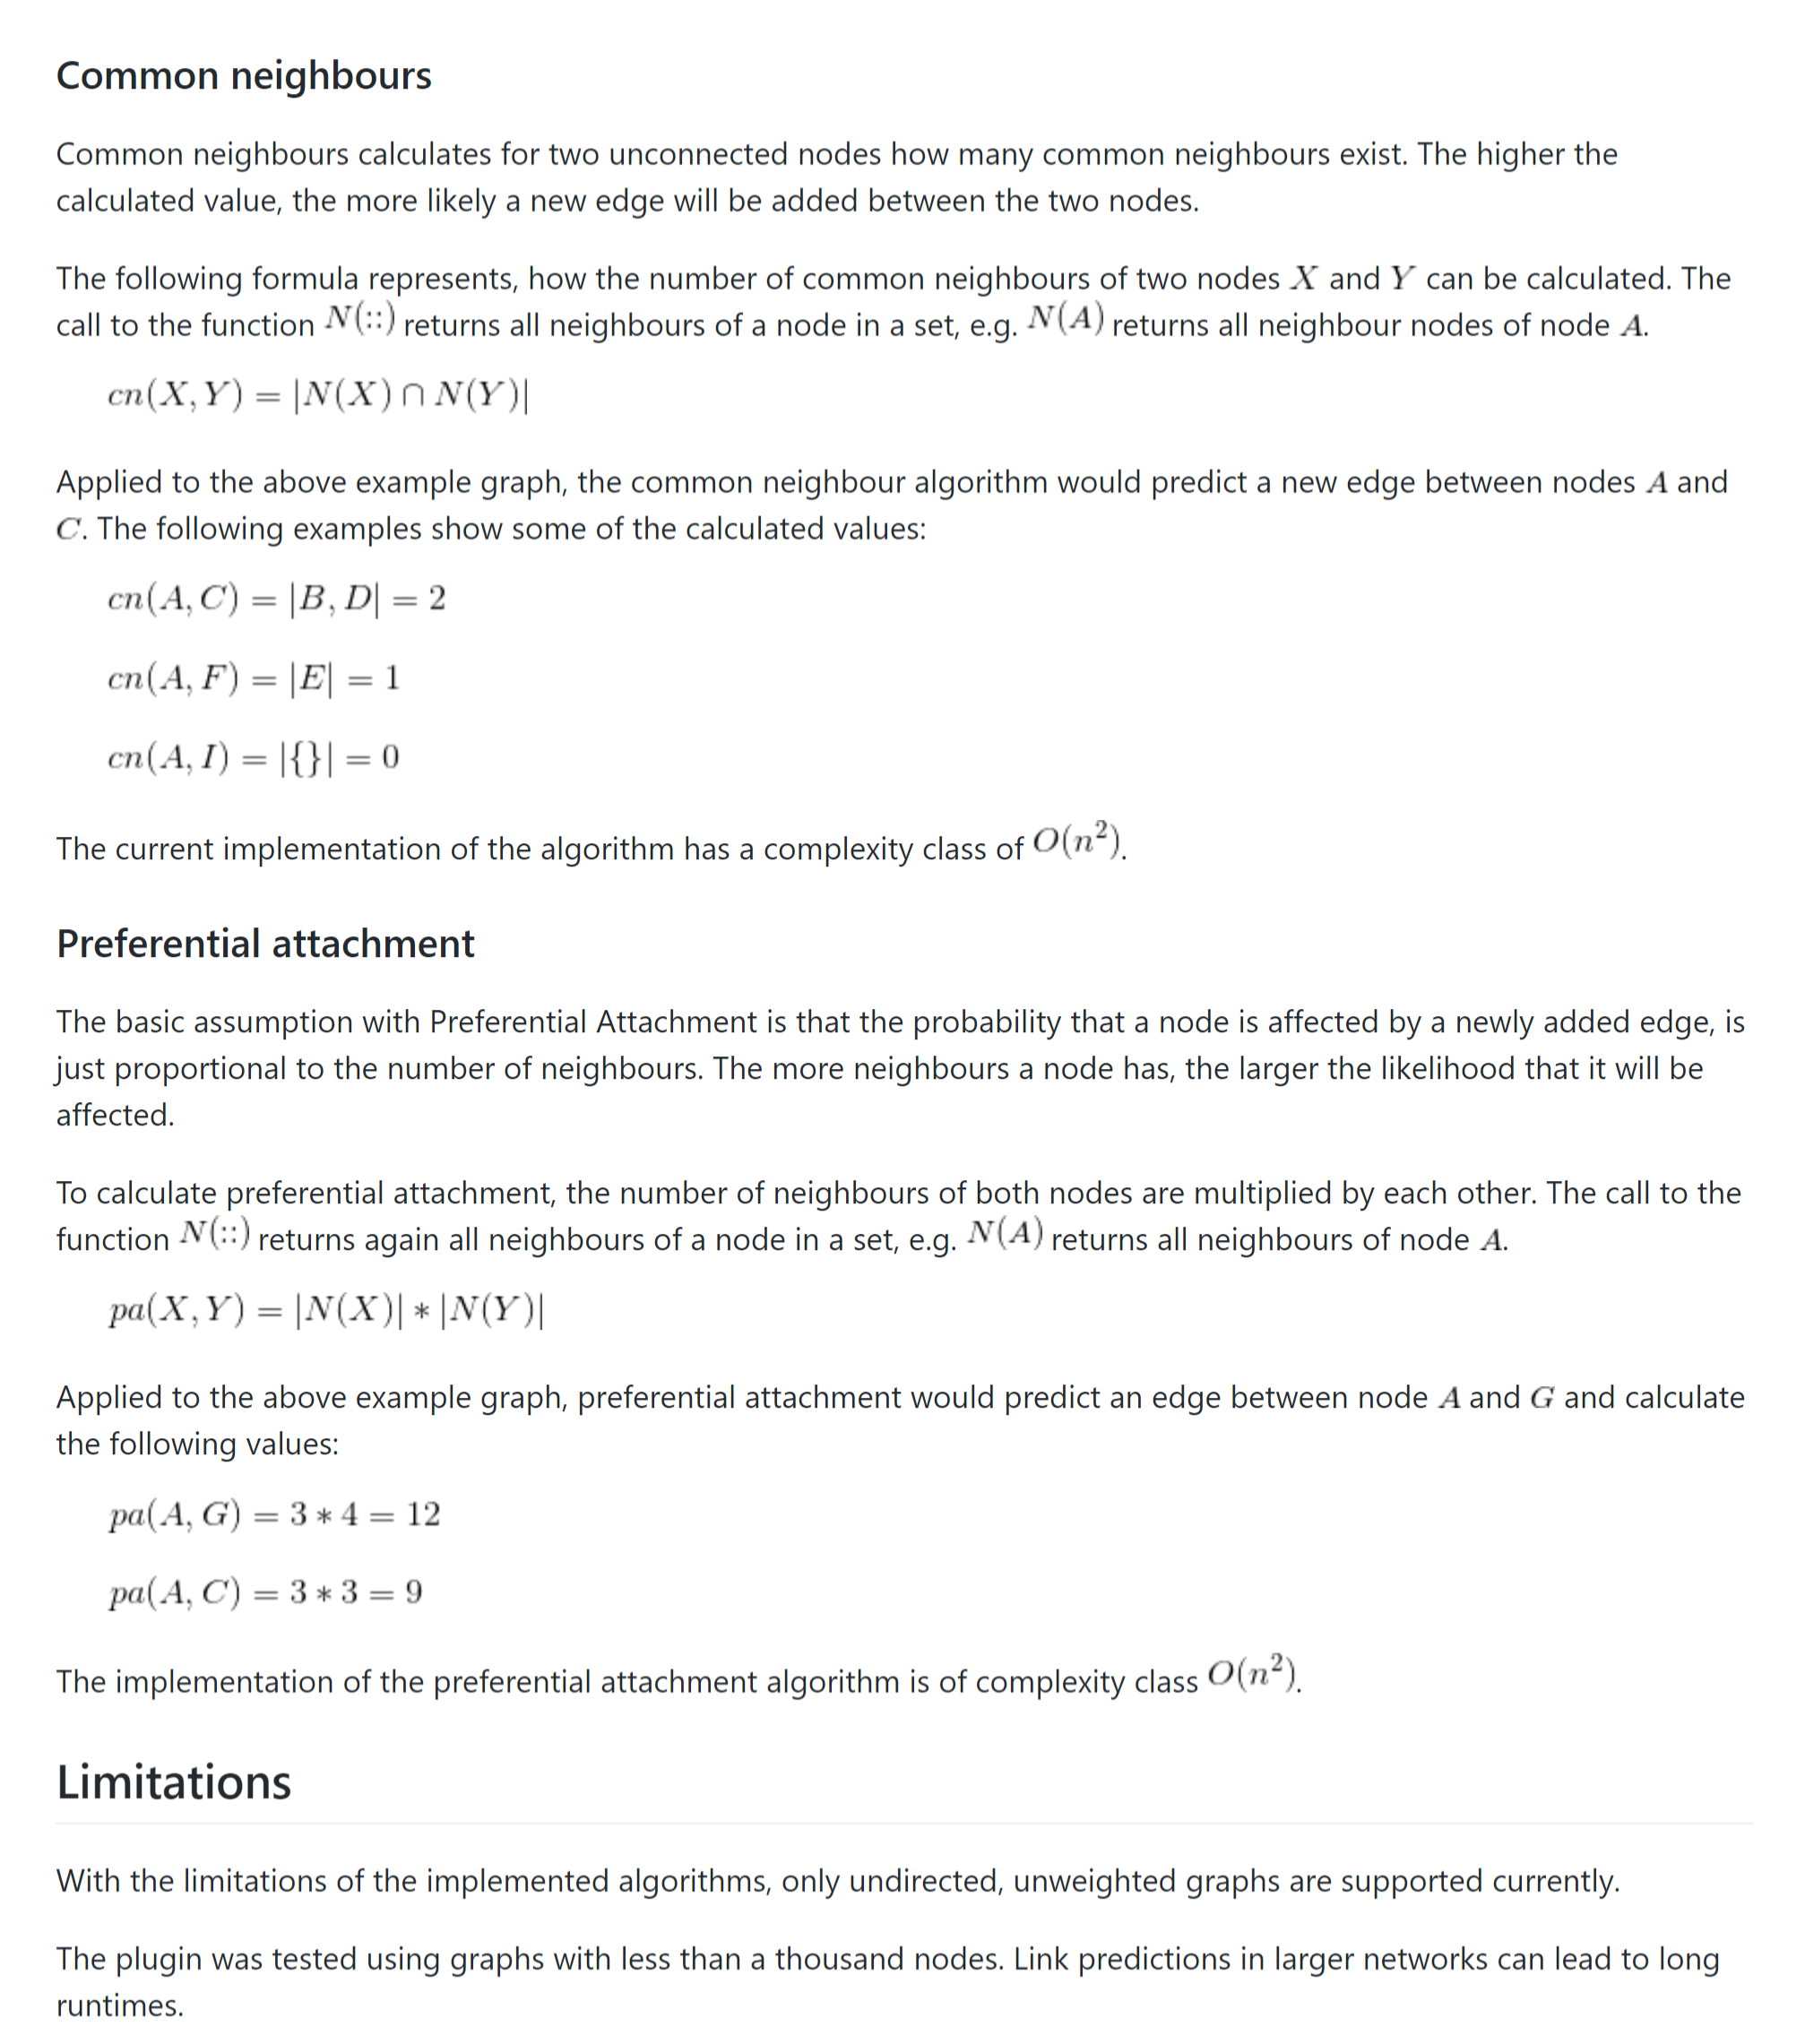
\includegraphics[width=\textwidth]{resources/readme_pt3.png}

%TODO: Add Exception/Error to Glossar




% TODO Use form of Hochschule für Technik
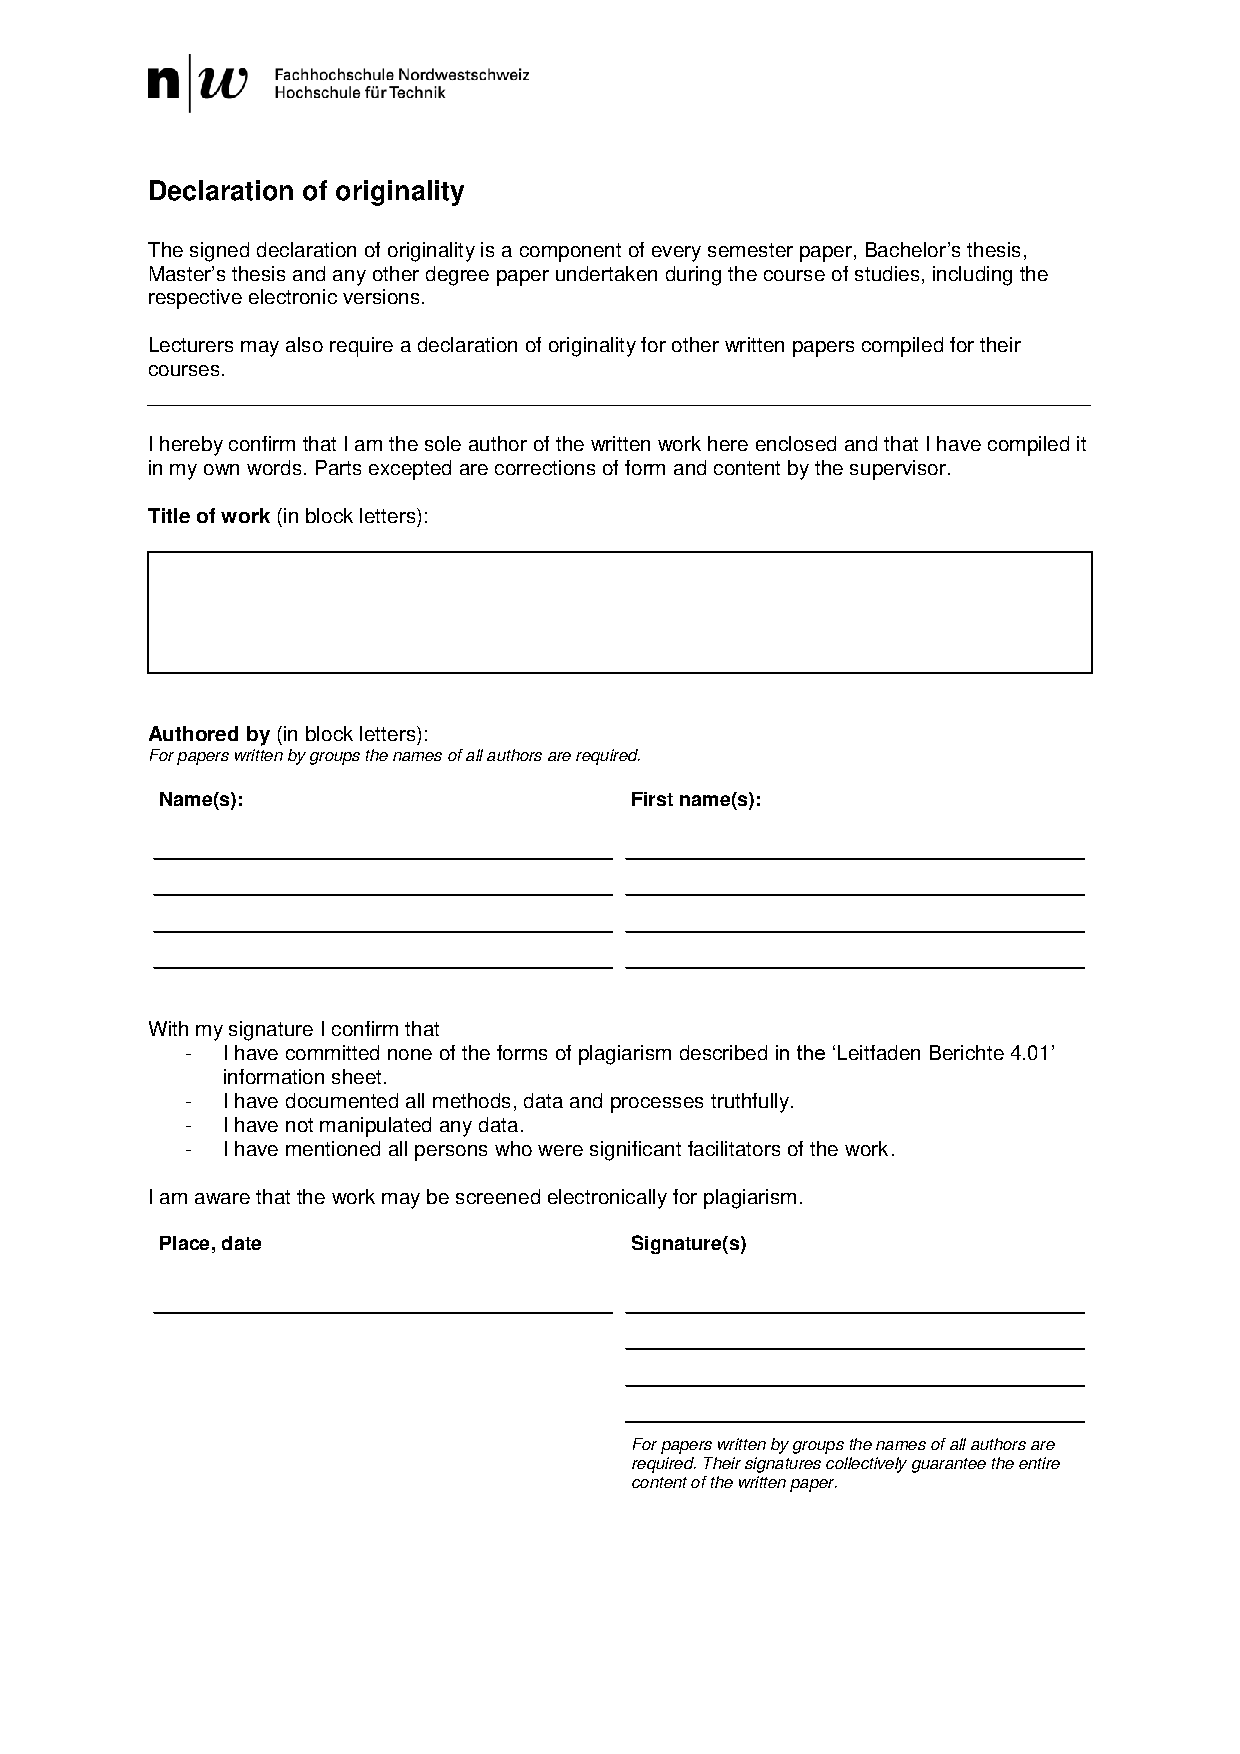
\includepdf[pages={-}]{resources/declaration-originality.pdf}

\end{document}
